% Capability Exposure Accounting, version 4.0.3. Compiler: pdfLaTeX; bibliography: BibTeX.
\documentclass[pdflatex,sn-mathphys-num]{sn-jnl}
\usepackage[T1]{fontenc}
\usepackage[utf8]{inputenc}
\usepackage{amsmath,amssymb,amsfonts}
\usepackage{graphicx,booktabs,tabularx,array,longtable}
\usepackage{fvextra,tikz,xurl,needspace}
\usetikzlibrary{arrows.meta,positioning}
\theoremstyle{plain}
\newtheorem{theorem}{Theorem}
\newtheorem{lemma}[theorem]{Lemma}
\newtheorem{proposition}[theorem]{Proposition}
\newtheorem{corollary}[theorem]{Corollary}
\theoremstyle{definition}
\newtheorem{definition}[theorem]{Definition}
\newtheorem{assumption}{Assumption}
\newtheorem{observation}{Model-checking observation}
\newcommand{\Cl}{\operatorname{Cl}}
\newcommand{\F}{\mathbb{F}}
\newcommand{\Adv}{\operatorname{Adv}}
\newcommand{\rk}{\operatorname{rank}}
\newcommand{\im}{\operatorname{im}}
\newcommand{\pk}{\mathsf{pk}}
\newcommand{\sk}{\mathsf{sk}}
\newcommand{\code}[1]{\texttt{#1}}
\newcolumntype{Y}{>{\raggedright\arraybackslash}X}
\emergencystretch=2em
\hypersetup{hidelinks,bookmarksdepth=2,pdftitle={Capability Exposure Accounting for Threshold-Based Encrypted Backup Recovery},pdfauthor={Samarjeet Malik and Shaurya Pratap Singh}}
\begin{document}
\raggedbottom
\title[Capability Exposure Accounting]{Capability Exposure Accounting for Threshold-Based Encrypted Backup Recovery}
\author[1]{\fnm{Samarjeet} \sur{Malik}}
\author[2]{\fnm{Shaurya Pratap} \sur{Singh}}
\affil[1]{\orgname{Ashoka University}}
\affil[2]{\orgname{Indian Institute of Science}}
\abstract{\unboldmath Deleting a custodian's local secret need not revoke an encrypted backup's recovery capability: copied credentials, recorded capsules, refreshed sharings and archive authorities can preserve access. We model surviving capabilities as a typed conjunctive closure over affine observations. A leakage subspace of dimension $\rk[A\ B]-\rk B$ decides reconstruction, privacy on arbitrary seed domains, and exact marginal and conditional mutual information. Erasure planning is witness hitting. It is linear-time on read-once exposure formulas, NP-hard with weighted thresholds, solvable in $n^{O(2^G)}$ time for $G$ generations with reused credentials, and APX-hard when each reused credential serves at most three generations. For independently randomized Pedersen-committed generations the budget counts touched indices, not complete pairs. A temporal accounting theorem, checked against exact rank computation on 3,000 random histories, separates algebraic from delivery independence. Our main cryptographic result is a restricted-adaptive composition theorem for the HPKE/HMAC/AEAD profile. The adversary may expose slots, bank roots and coordinates adaptively. Every term of the bound is multiplied by the size $L$ of a guessing space of late-exposure patterns of the target's generations: $L=1$ when exposure is forward-ordered and $L=16$ for one 3-of-5 generation. For the specific delivery map in which each holder's bank is reused across generations, the reachable patterns have an exact count that is far smaller (3,991 instead of 970,299 for three 5-of-7 generations); for other delivery maps the general factor applies. The accounting separates object-level requests from chunk-level AEAD calls, fixes every advantage convention, and charges the coincidence of independently derived object keys, which would reuse a key-byte and nonce pair. A reference data layer built on maintained primitives showed that the profile must bind a final-chunk flag to detect truncation. Within this proof approach, removing $L$ would require a receiver selective-opening guarantee for the capsule encryption, or a different construction; full adaptivity is not claimed. Lifecycle verification adds liveness under strong fairness, which shows that erasure progress requires terminating hung decryption workers, and a mobile-adversary renewal model. A Python transcription of the TLA+ lifecycle reproduces TLC's state counts exactly; checking the reference kernel against it on 2,000 seeded schedules found four classes of divergence in the earlier kernel and none after the fix. Results are relative to declared operations and affine views; they do not certify physical erasure.}
\keywords{Capability exposure, encrypted backup, threshold recovery, cryptographic erasure, linear secret sharing, selective opening, adaptive corruption, refinement, TLA+}
\maketitle


\section{Introduction}\label{sec:intro}

Encrypted recovery creates durable access to data whose live communication keys may already have evolved. Losing every message device is recoverable only if some external capability survives. Erasing access to an old record requires that the adversary's permitted later view contain no sufficient surviving path. These are different questions: legitimate recoverability is a property of available honest authorities, whereas confidentiality after compromise concerns the authority and material actually disclosed to the adversary.

Several distinctions determine the outcome. A record's birth epoch is unchanged when it is placed in a newer snapshot. Deleting a cached share does not remove a recorded share capsule's recipient key. Deleting an honest device's key does not remove a previously copied key. Refreshing sharing polynomials does not renew the credentials that decrypt their capsules. An independent archival service adds a recovery route rather than removing the ordinary route's limitations. An authentic approval can still authorize an attacker-controlled recipient through a genuine mistake.

The underlying mechanisms are established. Revocable backup and ephemerizer systems exploit deliberate key destruction~\cite{boneh1996,perlman2007}; policy-based secure deletion composes key erasure along a policy graph~\cite{cachin2013}; proactive sharing, APSS and CODEX address distributed custody under explicit compromise assumptions~\cite{ostrovsky1991,herzberg1995,zhou2005,marsh2004}; CKS and GKP give cryptographic treatments of persistent key access~\cite{dodis2024,dodisstandard2024,backendal2026}. Our question is narrower: how to account, after an arbitrary finite history, for every surviving route to a threshold-shared recovery seed, and what that accounting implies for erasure, renewal and operation.

\paragraph{Research questions.}
RQ1 (capability accounting): which surviving capabilities, including alternate and recorded paths, suffice for reconstruction or for information leakage after a specified exposure? RQ2 (temporal exposure): which exposures can share refresh, recipient-credential renewal, seed renewal and capsule re-encryption heal, and which are irreversible? RQ3 (joint progress): which parameter and service conditions permit recovery, approval, deletion progress and ordered operation despite withholding and outages?

\paragraph{Contributions and their status.}
We separate new results from specializations of known ones. Items marked v4 are new in this version; the rest were established in v3.0.0 and re-audited here.
\begin{enumerate}
\item A leakage-subspace characterization of affine views (Theorem~\ref{thm:leakage}). v4 adds exact marginal and conditional leakage with a chain rule (Corollary~\ref{cor:condleak}). It also shows that uniform masks are necessary and that the adaptive corollary needs a transcript-measurable acceptance predicate. All of this is elementary linear algebra used as a single decision object.
\item An erasure analysis (Section~\ref{sec:erasure}). Witness hitting and read-once evaluation are known from attack-tree analysis~\cite{mauw2005,lopuhaa2022}. v4 corrects the runtime claim, which now uses linear-time selection. It adds NP-hardness and a pseudo-polynomial algorithm for weighted thresholds, an $n^{O(2^G)}$ algorithm for $G$ generations with reused credentials, and APX-hardness when each reused credential serves at most three generations.
\item A corrected joint-generation theorem counting touched indices (Theorem~\ref{thm:generations}) and a blockwise lemma (Lemma~\ref{lem:block}).
\item A temporal exposure-accounting theorem and healing classification (Theorem~\ref{thm:temporal}). v4 validates it against exact rank computation on random multi-epoch histories and shows that the independence hypothesis cannot be dropped.
\item (v4) A restricted-adaptive composition theorem (Theorem~\ref{thm:adaptive}) with explicit hybrids. Every term is multiplied by the size $L$ of a guessing space that contains every late-exposure pattern a fresh run can produce, and $L=1$ under forward-ordered exposure. Within this approach, removing $L$ would need a receiver selective-opening guarantee, which ordinary IND-CCA is not known to provide. The v3 selective theorem's AEAD and identifier-collision accounting is corrected, and the PRF, key and chunk-call counts are corrected (v4.0.1 and v4.0.2). v4.0.2 adds a closed-form reachable pattern count for reused banks (Proposition~\ref{prop:patterns}).
\item Committee feasibility (Propositions~\ref{prop:holders}--\ref{prop:committees}). v4 adds domain-correlated corruption (Proposition~\ref{prop:domains}).
\item Formal evidence (Section~\ref{sec:formal}). v4 adds strong-fairness liveness for the lifecycle, a mobile-adversary renewal model, and a Python transcription of the TLA+ lifecycle validated by exact state-count agreement with TLC. It also adds bounded refinement-conformance testing of the kernel against that transcription. This found four divergence classes in the v3 kernel, now fixed. It is testing, not a refinement proof.
\end{enumerate}
None of these is a new cryptographic primitive, and we make no priority claim for the linear-sharing, monotone-derivation, hitting-set or guessing-based foundations~\cite{karchmer1993,panjwani2007}.

\section{Position relative to prior work}\label{sec:related}

\paragraph{Deletion and custody.}
Boneh--Lipton's revocable backups and Perlman's ephemerizers are direct predecessors to cryptographic forgetting with externally held temporary keys~\cite{boneh1996,perlman2007}. Cachin et al.\ give a cryptographic model of policy-based secure deletion in which protection classes are erased according to a policy expressed as a directed acyclic graph, together with a filesystem prototype~\cite{cachin2013}. Their policy graph is the closest predecessor of our witness structures. The differences are in what is shared and what survives. Our roots include threshold-shared seeds observed through affine views, adversary copies that persist across later honest operations, and multiple independently randomized generations. The witness predicate is therefore sometimes a rank condition rather than a Boolean gate. We do not claim a stronger deletion definition than theirs. Reardon, Basin and Capkun systematize deletion on physical media~\cite{reardon2013}; we inherit their warning that logical key removal does not certify physical erasure. FadeVersion addresses assured deletion with version dependencies in cloud backup~\cite{rahumed2011}; our implementation is a lifecycle reference, not a competing backup system.

\paragraph{Proactive custody and share refresh.}
Shamir and Pedersen sharing supply the algebra~\cite{shamir1979,pedersen1991}. Ostrovsky and Yung introduced the mobile adversary~\cite{ostrovsky1991}; proactive secret sharing and APSS bound compromise per refresh window and implement transitions~\cite{herzberg1995,zhou2005}; CODEX combines authorized secret distribution with Byzantine quorums~\cite{marsh2004}. Our temporal theorem is an accounting statement about a complete recorded history under honest independent generation. It is not a refresh protocol, and it does not provide APSS's transition guarantees. What it adds is explicit: share refresh heals cross-period accumulation of share disclosures only if each new generation is also delivered along paths the adversary cannot open. We use ``proactive'' only for the cited protocols; our results assume honest generation and establish no refresh protocol or corruption-window guarantee. A refresh whose capsules are addressed to a copied bank is algebraically fresh and operationally exposed.

\paragraph{Compact and evolving persistent keys.}
ROM-CKS gives line and interval constructions preserving compatible application security; its adaptive simulation uses noncommitting techniques~\cite{dodis2024}. The standard-model follow-up shows the original preservation objective cannot be instantiated as stated there and recovers derived keys with selective definitions~\cite{dodisstandard2024}. GKP/Grappa provides persistent interval access and post-compromise evolution under its group model~\cite{backendal2026}. These comparisons are carried over from the v2.0.0 inspection of the cited full versions and were not re-audited in this revision. Our independent-slot array is a less compact component with direct exposure accounting, not a substitute for either.

\paragraph{Authenticated recovery and cloud storage.}
Kintsugi uses password-authenticated threshold recovery with non-Byzantine nodes and per-interval share-disclosure bounds~\cite{ma2025}. Juicebox combines threshold OPRFs, secret sharing and self-destructing guess counters across independent realms~\cite{trapp2025}. SafetyPin and SVR3 provide deployed hardware-split recovery~\cite{dauterman2020,connell2024}. Janneck--Riepel refine encrypted cloud-storage security with adaptive corruptions and network adversaries~\cite{janneck2026}. These systems answer authentication and deployment questions that we do not; we assume authenticated bootstrap and a verified log. Their designs are natural targets for the accounting, not objects it improves upon.

\paragraph{Adaptive corruption and selective opening.}
Encrypting secret shares to many receivers and then letting the adversary corrupt receivers after it has seen the ciphertexts is a receiver selective-opening setting. Bellare, Hofheinz and Yilek introduced selective-opening security and its possibility and impossibility results~\cite{bellare2009}. Hazay, Patra and Warinschi define receiver selective-opening security and obtain indistinguishability-based security from a variant of noncommitting encryption~\cite{hazay2015}. Noncommitting encryption is the classical route to adaptive security~\cite{canetti1996}. Panjwani's generalized selective decryption and the framework of Jafargholi et al.\ show how guessing can be confined to the parts of an adaptive choice that matter, reducing the loss~\cite{panjwani2007,jafargholi2017}. Our restricted-adaptive theorem uses the plain form of that idea: it guesses only the late-exposure pattern of the target seed's generations. Alwen et al.\ analyse HPKE's authenticated mode~\cite{alwen2021}. We use IND-CCA security of the Base mode used here~\cite{rfc9180} as an assumption, and do not claim selective-opening security for it.

\paragraph{Attack trees.}
Minimum-cost attacks on tree-structured AND/OR attack trees are computed bottom-up~\cite{mauw2005}; on DAG-structured trees the problem is NP-hard~\cite{lopuhaa2022}. Minimum erasure is a minimum attack on the dual formula (swap AND with OR, threshold $k$ of $m$ with $m-k+1$ of $m$). Section~\ref{sec:erasure} uses these facts and claims only their interpretation for credential reuse.

\begin{table}[htbp]
\caption{Comparison of problem scope. Entries describe the cited interfaces as inspected; ``this paper'' entries are relative to declared operations and affine views.}\label{tab:comparison}
\centering\footnotesize
\begin{tabularx}{\linewidth}{@{}p{.15\linewidth}YYYY@{}}\toprule
Work & Problem & Threat model & Key evolution / erasure & Evidence\\\midrule
Boneh--Lipton; Perlman & Revocable backup; assured delete & Later key-holder compromise & Destroy encrypting keys & Design\\
Cachin et al. & Policy-based deletion & Cryptographic deletion game & DAG policy over erasable keys & Proofs; filesystem prototype\\
PSS; APSS; CODEX & Proactive custody (refresh protocols) & Mobile/Byzantine; asynchronous (APSS) & Share refresh protocols & Proofs; systems\\
CKS; GKP & Persistent key access & ROM adaptive / standard selective; group model & Compact derivation; interval progression & Proofs\\
Kintsugi; Juicebox; SafetyPin; SVR3 & PIN/password recovery & Non-Byzantine nodes; realms; HSM trust & Guess limits; self-destruct; hardware & Systems; deployment\\
Janneck--Riepel & Cloud storage & Adaptive corruption, network adversary & Modular & Proofs\\
SOA / NCE / GSD & Opening after encryption & Adaptive receiver corruption & --- & Proofs (generic)\\
This paper & Exposure accounting for threshold-shared seeds & Declared operations; affine views; copies persist; restricted-adaptive composition & Generations, banks, archives, renewal & Theorems; TLC; refinement testing\\\bottomrule
\end{tabularx}
\end{table}

What remains new is therefore modest and specific. It consists of an exact affine-leakage accounting for threshold recovery histories, the corrected generation criterion, and the temporal healing classification. It also includes the complexity map of erasure planning under credential reuse, a restricted-adaptive composition theorem whose loss factor is the size of a late-exposure guessing space, and the checked lifecycle and barrier models with tested kernel conformance. Broader claims about a general audit method would require external validation that we do not have.


\section{Exposure model}\label{sec:model}

\subsection{State, locations and compromise}
A record has immutable birth epoch $e$. Its sharing generations $g$ may change without changing $e$. Snapshot version $v$ is a container identifier, not a birth epoch. Let $j$ be the committed recovery frontier, $W$ an ordinary retention window, and $L$ the effective deletion floor. Ordinary recovery covers promised records with $j-W+1\le e\le j$; advancing $j$ requires completed barriers for older protected records.

At time $t$ the system state is $(H_t,A_t,P_t,\Pi_t,J_t)$: honest located capabilities, adversary-owned knowledge, public recorded material, lifecycle/policy state, and pending work. The atom universe $V$ tags each atom with role, location, epoch, generation, holder and bank version.

\begin{assumption}[Origin tagging]\label{ass:origin}
Honest locations and adversary copies are distinct atoms, even when they derive the same usable value. Deletion removes an honest atom; it never removes an atom of $A_t$. Consequently $A_t\cap H_t=\varnothing$, and $A_t$ is monotone under all honest operations.
\end{assumption}

The exposure map specifies which honest locations a corruption or later snapshot discloses. An ordinary-compromise claim may exclude an independent archive authority; a claim about erasure across all recovery routes must include it. We distinguish four compromise interfaces. \emph{Identity compromise} supplies signing authority and malicious voting, without a data slot. \emph{Device compromise} supplies the enumerated local slots, caches, buffers and retained wrappers. \emph{Capability disclosure} supplies a particular copied pair, slot, response or derivation ancestor. \emph{Recovery-authority compromise} supplies an alternate route such as an archive key or reconstructed client seed. Table~\ref{tab:oracles} lists the trace interfaces.

\begin{table}[htbp]
\caption{Trace interfaces and returned material. A real device disclosure may cross several categories when keys are co-resident.}\label{tab:oracles}
\centering\footnotesize
\begin{tabularx}{\linewidth}{@{}p{.26\linewidth}Y@{}}\toprule
Interface & State or observation supplied\\\midrule
Setup / Publish & Honest bank directories, epoch/generation parameters, public manifests, commitments and recorded capsules\\
CopySlot$(h,b,e)$ & The present matching private slot, or failure if absent; an earlier copy remains in adversary state\\
CopyBankCapability & Every retained slot in that bank snapshot, including future periods; no signing authority\\
CorruptDevice & Stored slots, cached shares, wrapper roots and volatile responses, including in-flight worker state; stored signing keys also count as identity compromise\\
CorruptIdentity & Specified signing/policy keys and malicious voting, without a data slot\\
CopyPair / CopyResponse & Declared pair coordinates or recorded response material; deliveries are never retracted\\
CorruptRecoverer & Reconstructed seeds, available pairs, plaintext outputs, session state and buffers\\
CorruptArchive & The specified archival root/slots and their recorded envelopes\\
Expire / Crash / Restart & Lifecycle transitions; old snapshots must pass the nonrollback anchor\\
FinalSnapshot & The honest-origin fields allowed by the exposure map, followed by declared closure\\\bottomrule
\end{tabularx}
\end{table}

\subsection{Declared symbolic operations}
Let $\mathcal R$ contain typed rules $Q\Rightarrow v$ with conjunctive premise set $Q\subseteq V$. A recorded capsule \emph{and} its matching private slot derive the coordinates it encrypts. A wrapped slot \emph{and} its wrapping root derive the slot. A cached pair, exposed buffer or delivered response independently supplies coordinates. An archive capsule and its archive key derive the seed. A seed and an encrypted record derive record access. A signing identity alone derives no data.

Accessible observation atoms index rows of a matrix over $\F_p$. The closure adds conclusions of enabled rules and any registered seed atom linearly decodable from accessible rows, repeating until the least fixed point $\Cl_{\mathcal R}(K)$.

\begin{theorem}[Relative closure characterization]\label{thm:closure}
For a finite atom universe and fixed typed rules and linear decoders, $v\in\Cl_{\mathcal R}(K)$ if and only if $v$ has a finite derivation from $K$ using those operations. The fixed-point procedure terminates after at most $|V|$ productive rounds, and $\Cl_{\mathcal R}$ is monotone: $K\subseteq K'$ implies $\Cl_{\mathcal R}(K)\subseteq\Cl_{\mathcal R}(K')$.
\end{theorem}
\begin{proof}
Every added Horn conclusion has a derivation from already derived premises, and every linear-decoder step has a row-combination certificate; induction over rounds gives soundness. Conversely, induction over a finite derivation tree places its root in the fixed point. Each productive round adds an atom of the finite universe. Monotonicity holds because every operation's enabling condition is monotone in the available atoms: a premise set remains present, and a row span only grows.
\end{proof}

Completeness is relative to the inventory: an unlisted disk root or unmodeled client side effect is not excluded by calling the closure complete.

\begin{figure}[htbp]
\centering
\resizebox{\linewidth}{!}{%
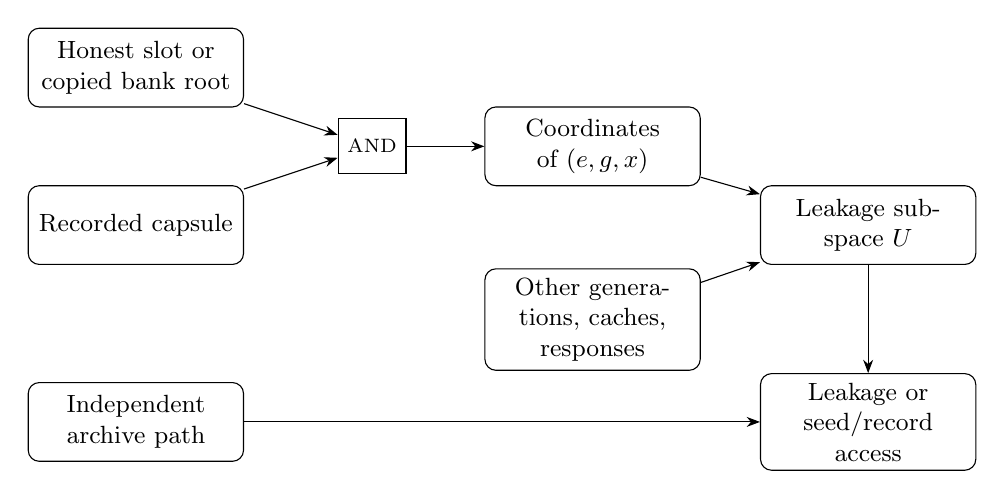
\begin{tikzpicture}[>=Stealth,box/.style={draw,rounded corners,align=center,font=\small,text width=25mm,minimum height=10mm},gate/.style={draw,rectangle,align=center,font=\scriptsize,minimum size=7mm}]
\node[box] (root) at (0,4.5) {Honest slot or copied bank root};
\node[box] (cap) at (0,2.5) {Recorded capsule};
\node[gate] (and) at (3,3.5) {AND};
\node[box] (pair) at (5.8,3.5) {Coordinates of $(e,g,x)$};
\node[box] (obs) at (5.8,1.3) {Other generations, caches, responses};
\node[box] (linear) at (9.3,2.5) {Leakage subspace $U$};
\node[box] (archive) at (0,0) {Independent archive path};
\node[box] (seed) at (9.3,0) {Leakage or seed/record access};
\draw[->] (root)--(and);\draw[->] (cap)--(and);\draw[->] (and)--(pair);
\draw[->] (pair)--(linear);\draw[->] (obs)--(linear);\draw[->] (linear)--(seed);
\draw[->] (archive)--(seed);
\end{tikzpicture}}
\caption{A capability hypergraph, not edge reachability. Conjunctive openings feed an affine observation module whose leakage subspace decides both reconstruction and privacy. A bank root reused across generations feeds several conjunctions; this sharing is what makes minimum erasure hard (Section~\ref{sec:erasure}).}\label{fig:capabilities}
\end{figure}


\section{Reconstruction and leakage}\label{sec:leakage}

Let the protected seeds be $S\in D\subseteq\F_p^k$. Let $R$ be uniform on $\F_p^r$ and independent of $S$, containing every sharing coefficient and blinder. For a fixed choice of observations, the accessible view is
\begin{equation}\label{eq:view}
 Y=AS+BR,\qquad A\in\F_p^{m\times k},\ B\in\F_p^{m\times r}.
\end{equation}
Every observation source and public affine quantity must appear as a row. Seeds whose values are given (conditioning) are substituted and their contribution subtracted; seeds that are unknown but not uniform are never treated as masks.

\begin{definition}[Leakage subspace]
$U=\{\lambda A:\lambda\in\F_p^{1\times m},\ \lambda B=0\}\subseteq\F_p^{1\times k}$. Let $M\in\F_p^{d\times k}$ have rows forming a basis of $U$, where $d=\dim U$.
\end{definition}

\begin{theorem}[Leakage subspace]\label{thm:leakage}
For the view~\eqref{eq:view}:
\begin{enumerate}
\item $\dim U=\rk[A\ B]-\rk B$.
\item For $s,s'\in\F_p^k$, the conditional laws of $Y$ given $S=s$ and $S=s'$ are equal if and only if $Ms=Ms'$; otherwise their supports are disjoint.
\item (Privacy) $Y$ is independent of $S$ on $D$ if and only if $M(s-s')=0$ for all $s,s'\in D$. If $D=D_1\times\cdots\times D_k$ with every $|D_i|\ge2$, this holds if and only if $U=0$, equivalently $\rk[B\ A]=\rk B$.
\item (Reconstruction) On $D=\F_p^k$, a functional $cS$ is a deterministic function of $Y$ if and only if $c\in U$, equivalently $(c,0)\in\operatorname{rowspan}[A\ B]$. It is then computed by a linear decoder $\lambda Y$. On a restricted $D$, $cS$ is determined by $Y$ if and only if $cs=cs'$ whenever $s,s'\in D$ and $Ms=Ms'$, which may hold with $c\notin U$.
\item (Leakage) $I(S;Y)=H(MS)\le d\log_2p$ bits, with equality when $S$ is uniform on $\F_p^k$.
\end{enumerate}
\end{theorem}
\begin{proof}
(1) The left kernel of $B$ has dimension $m-\rk B$. The map $\lambda\mapsto\lambda A$ on it has kernel equal to the left kernel of $[A\ B]$, of dimension $m-\rk[A\ B]$. Its image $U$ has dimension $(m-\rk B)-(m-\rk[A\ B])$.

(2) Given $S=s$, $Y$ is uniform on the coset $As+\im B$. Two cosets are equal or disjoint, and equal iff $A(s-s')\in\im B$. Since $\im B$ is exactly the set of vectors annihilated by every $\lambda$ with $\lambda B=0$, this holds iff $\lambda A(s-s')=0$ for all such $\lambda$, that is, iff $M(s-s')=0$.

(3) The first claim is (2) applied to all pairs in $D$. For a product domain, choose $s,s'$ differing only in coordinate $i$ by a nonzero $\delta$; then $M(s-s')=\delta M e_i$, so privacy forces every column of $M$ to vanish, i.e.\ $U=0$. Conversely $U=0$ gives privacy on any domain. Finally $U=0$ iff every column of $A$ lies in $\im B$ iff $\rk[B\ A]=\rk B$.

(4) If $c=\lambda A$ with $\lambda B=0$ then $\lambda Y=cS$. Conversely, suppose $cS$ is a function of $Y$ on $\F_p^k$. Let $s-s'\in\ker M$. By (2) the two conditional laws have the same support, so some $y$ occurs under both; hence $cs=cs'$. Therefore $c$ annihilates $\ker M$, so $c\in(\ker M)^\perp=\operatorname{rowspan}M=U$. The equivalence with $(c,0)\in\operatorname{rowspan}[A\ B]$ is the definition of $U$. The restricted-domain statement is (2) restricted to $D$.

(5) $MS=\Lambda Y$ for the matrix $\Lambda$ whose rows are the chosen $\lambda$'s, so $MS$ is a function of $Y$. By (2), the law of $Y$ given $S$ depends on $S$ only through $MS$. Hence $S\to MS\to Y$ is a Markov chain with $MS$ a function of both $S$ and $Y$, and $I(S;Y)=I(S;MS)=H(MS)$. The bound is $|\F_p^d|$; uniform $S$ makes $MS$ uniform on $\F_p^d$ because $M$ has full row rank.
\end{proof}

Part~(4) corrects a dimensional imprecision in the v2.0.0 statement. The target vector is $(e_i,0)\in\F_p^{1\times(k+r)}$, the unit vector on the seed coordinate concatenated with zeros on every mask coordinate; it is not a ``unit row'' of $[A\ B]$. On full domains linear decoding is not a restriction: no decoder of any kind does better. On restricted domains it is. The selected profile embeds 32-byte seeds in a 384-bit field, which is such a domain. For example, with $Y=S_0+2S_1$ over $\F_5$ and $S\in\{0,1\}^2$, $Y$ determines both seeds although $e_0\notin U$. Part~(3) also covers correlated seeds: if the support is $\{s:s_0=s_1\}$, the observation $S_0-S_1$ violates the rank test but leaks nothing. The relation-only example $Y=S_0+S_1$ illustrates the converse gap: it reconstructs neither coordinate, yet $d=1$ and it leaks $\log_2p$ bits.

\begin{corollary}[Marginal and conditional leakage]\label{cor:condleak}
Let the seeds be independent and uniform on $\F_p^k$, split into a target block $T$ and the rest $K$. Let $\pi_T$ be the coordinate projection onto $T$, and let $U_{T}=\{u\in U:u_K=0\}$. Then
\[
 I(S_T;Y)=\dim U_T\cdot\log_2p,\qquad I(S_T;Y\mid S_K)=\dim\pi_T(U)\cdot\log_2p,
\]
and $\dim U=\dim\pi_T(U)+\dim\{u\in U:u_T=0\}$, which is the chain rule $I(S;Y)=I(S_K;Y)+I(S_T;Y\mid S_K)$.
\end{corollary}
\begin{proof}
Given $S_K=s_K$, substitute it and subtract; the remaining view is $A_TS_T+BR$, whose leakage space is $\{\lambda A_T:\lambda B=0\}=\pi_T(U)$. Apply Theorem~\ref{thm:leakage}(5) for each $s_K$. For the marginal, the unknown uniform $S_K$ acts as an additional mask block, so the leakage space is $\{\lambda A_T:\lambda[B\ A_K]=0\}$, which is exactly $U_T$ read on the $T$ coordinates. The dimension identity is rank--nullity for $\pi_T$ restricted to $U$; its kernel is $\{u\in U:u_T=0\}$, the marginal leakage space of $S_K$.
\end{proof}

Uniform masks are necessary for the general coset characterization in Theorem~\ref{thm:leakage}(2), and hence for using the rank test as a privacy criterion without further analysis. If $R$ is uniform on a subspace spanned by the columns of $C$, replace $B$ by $BC$ and all statements hold. If $R$ has any other distribution, the rank test is no longer sound in general. For $Y=S+R$ over $\F_3$ with $R$ uniform on $\{0,1\}$, $U=0$ although the support of $Y$ depends on $S$. Particular non-uniform distributions may still give private views, for example when $A=0$; such cases need their own argument. Blinders in the profile are uniform in the full field, so this concerns only implementations that draw masks from a smaller range.

\begin{corollary}[Adaptive observations]\label{cor:adaptive}
Let an adversary with fixed coins choose each next observation row as a function of the answers so far, over a finite mask tape. A terminal transcript $\tau$ fixes matrices $A_\tau,B_\tau$. For allowed $s_0,s_1$ with $A_\tau(s_1-s_0)\in\im B_\tau$, $\Pr[\tau\mid S=s_0]=\Pr[\tau\mid S=s_1]$. Consequently, if acceptance is a function of $\tau$ that implies this condition, the accepted subdistributions agree, and so do the laws conditioned on acceptance whenever acceptance has positive probability (that probability is then the same for $s_0$ and $s_1$).
\end{corollary}
\begin{proof}
Pick $d$ with $B_\tau d=A_\tau(s_0-s_1)$. The map $R\mapsto R+d$ is a measure-preserving bijection of the mask tape. It sends every tape producing $\tau$ under $s_0$ to a tape producing the same answers under $s_1$, because each answered row of $\tau$ is a row of $[A_\tau\ B_\tau]$. Identical answers produce identical later row choices, so the whole transcript is preserved. The acceptance probabilities are sums of equal transcript masses, so conditioning on acceptance preserves equality.
\end{proof}

The translation argument needs exactly three things. First, every row choice and the stopping time must be functions of the visible prefix and fixed coins. Variable-length transcripts and seed-dependent scheduling through the answers are allowed. Second, the acceptance predicate must be a function of the transcript; for several targets it is applied to each seed difference in turn. Third, public metadata must be a function of the transcript or independent of the seed. If acceptance depends on challenger state outside the transcript, the corollary fails. For $Y=S+R$ over $\F_5$, accepting iff $R=0$ yields accepted transcripts that equal $S$, whereas the transcript predicate ``accept iff $Y\neq0$'' gives equal accepted masses $4/5$ for every seed. Nothing is claimed for rejected transcripts, or for observations outside~\eqref{eq:view}, such as ciphertext lengths or nonlinear client behavior.


\section{Erasure as witness elimination}\label{sec:erasure}

Fix public recorded facts $P$, immutable adversary copies $A_0$, and honest-origin facts $H$ eligible for the stated future snapshot. By Assumption~\ref{ass:origin}, $A_0\cap H=\varnothing$. A permitted deletion $D\subseteq H$ leaves roots $P\cup A_0\cup(H\setminus D)$. Let the bad predicate $F$ be either declared reconstruction of a target or failure of the privacy test of Theorem~\ref{thm:leakage} after closure, and let $\mathcal W_F$ be the inclusion-minimal $W\subseteq A_0\cup H$ with $F(P\cup W)=1$.

\begin{theorem}[Witness hitting]\label{thm:cuts}
Under Assumption~\ref{ass:origin}, a permitted deletion prevents $F$ if and only if it intersects every $W\in\mathcal W_F$. If some witness lies in $A_0$, no permitted deletion prevents $F$.
\end{theorem}
\begin{proof}
Both predicates are monotone in the root set: closure is monotone (Theorem~\ref{thm:closure}), and adding rows can only enlarge $U$, since a $\lambda$ with $\lambda B=0$ extends by zeros. If $W$ is not hit then $W\subseteq A_0\cup(H\setminus D)$ and $F$ holds. Conversely, if $F$ holds after deletion, remove roots from $A_0\cup(H\setminus D)$ until a minimal witness remains. It avoids $D$ because $D\cap A_0=\varnothing$. A witness inside $A_0$ cannot be hit.
\end{proof}

Without origin tagging the theorem is false. If an atom lies in both $A_0$ and $H$, deleting the honest copy ``hits'' a witness that still survives through the adversary's copy. The fix is the tagging assumption, or replacing $H$ by $H\setminus A_0$.

\begin{definition}[Exposure formula]
An exposure formula is a monotone formula over roots built from AND, OR and threshold gates $\mathrm{THR}_k$, whose value is $F$. It is read-once if every root labels exactly one leaf. A root has deletion cost $w\in\mathbb{Z}_{\ge0}$, or $w=\infty$ if it is immutable (public, copied, or an undeletable authority).
\end{definition}

For independently randomized generations with pointwise disclosures, Theorem~\ref{thm:generations} below shows that privacy failure is the formula $\bigvee_g\mathrm{THR}_{t_g}(\tau_{g,x}:x)$. Here $\tau_{g,x}$ is the OR of the sources that touch index $x$ of generation $g$: a copied pair, a response, or the conjunction of a recorded capsule with a slot path.

\begin{proposition}[Read-once exposure; known recurrence]\label{prop:readonce}
For a read-once exposure formula, the minimum deletion cost $c(\cdot)$ that falsifies it satisfies $c(\text{leaf})=w$, $c(\wedge_i f_i)=\min_i c(f_i)$, $c(\vee_i f_i)=\sum_i c(f_i)$, and $c(\mathrm{THR}_k(f_1,\dots,f_m))$ equal to the sum of the $m-k+1$ smallest $c(f_i)$. The last value is $0$ if $k>m$ and $\infty$ if $k\le0$. With deterministic linear-time selection~\cite{blum1973} at threshold gates, $c$ is computable with $O(N)$ comparisons and $O(N)$ additions on the extended integers $\mathbb{Z}_{\ge0}\cup\{\infty\}$, and $O(N)$ memory, for a formula with $N$ nodes and edges. Sorting instead gives $O(N\log N)$ comparisons. Ties, zero costs and infinite costs need no special treatment beyond $x+\infty=\infty$.
\end{proposition}
\begin{proof}
Children of a read-once gate depend on disjoint roots, so a deletion falsifies the gate exactly when it falsifies the required children, and their costs add. AND needs one false child, OR needs all, and $\mathrm{THR}_k$ of $m$ needs $m-k+1$ false children, cheapest first. The sum of the $m-k+1$ smallest values is obtained by selecting the $(m-k+1)$-th smallest element in $O(m)$ time, then summing the values below it and the required number of ties. Summing over gates gives $O(N)$. This is the bottom-up minimal-attack computation for the dual tree~\cite{mauw2005,lopuhaa2022}.
\end{proof}

The v3 statement called the procedure linear-time while sorting at threshold gates, which costs $O(m\log m)$ per gate; the selection-based bound above removes that inconsistency.

\begin{proposition}[Weighted thresholds]\label{prop:weighted}
Consider a gate over $m$ children with positive integer weights $w_i$ and deletion costs $c_i\in\mathbb{Z}_{\ge0}\cup\{\infty\}$, true when the surviving weight is at least $k$. Let $W=\sum_iw_i$ and $R=W-k+1$, the weight that must be deleted. Computing the minimum falsifying cost is weakly NP-hard even for a single gate over leaves. It is computable in $O(mR)\subseteq O(mW)$ time and $O(R)$ space. A read-once formula of AND, OR, unweighted and weighted threshold gates is therefore solvable in $O(N+\sum_{\gamma}m_\gamma R_\gamma)$ time, the sum ranging over weighted gates $\gamma$.
\end{proposition}
\begin{proof}
If $R\le0$ the gate is already false (cost $0$); if $R>W$ it cannot be falsified (cost $\infty$). Otherwise the problem is a covering knapsack: choose children of total weight at least $R$ at minimum total cost. With $c_i=w_i$ the optimum equals $R$ iff some subset of the weights sums exactly to $R$, so an algorithm for the optimum decides subset sum, which is NP-complete~\cite{karp1972}; hence the problem is NP-hard. The dynamic program uses the state $F[x]$, the minimum cost of a chosen set with removed weight $\min(R,\cdot)=x$ for $0\le x\le R$, with $F[0]=0$. Processing child $i$ updates $F[\min(R,x+w_i)]\leftarrow\min(F[\min(R,x+w_i)],F[x]+c_i)$ for $x$ in decreasing order, and the answer is $F[R]$. This takes $O(mR)$ time and $O(R)$ space, which is pseudo-polynomial, so the hardness is weak. In a read-once formula each weighted gate uses its children's optima as item costs, because the children involve disjoint roots.
\end{proof}

\begin{proposition}[Reused credentials make erasure NP-hard]\label{prop:hard}
Minimum erasure is NP-hard and APX-hard even when every generation is a 2-of-2 sharing, every capsule is recorded and immutable, the only deletable roots are per-holder bank roots reused across generations, and each root is reused in at most three generations. With per-generation renewed banks, the same instances are read-once, and the minimum is one root per generation.
\end{proposition}
\begin{proof}
Reduce from vertex cover~\cite{karp1972}. For a graph $G=(V,E)$, let holders be vertices, each with one bank root of unit cost. Each edge $\{u,v\}$ becomes a 2-of-2 generation of the target seed, delivered to $u$ and $v$ under their banks. By Theorem~\ref{thm:generations} the seed leaks iff some generation has both indices touched, iff both endpoint banks of some edge survive. A deletion set prevents leakage iff it is a vertex cover, with equal cost, so the reduction preserves approximation ratios. Vertex cover is NP-hard and APX-hard~\cite{karp1972,dinur2005}, and it remains APX-complete on cubic graphs~\cite{alimonti2000}. A vertex of degree three gives a root reused in three generations. With renewed banks every root occurs once and Proposition~\ref{prop:readonce} applies.
\end{proof}

\begin{proposition}[Few generations]\label{prop:fewgen}
Consider $G$ generations of one seed over $n$ holders, each holder $h$ having one reused root of cost $w_h\in\mathbb{Z}_{\ge0}\cup\{\infty\}$, with recorded capsules and no other disclosures. Generation $g$ has holder set $H_g$ and threshold $t_g$, so it needs $d_g=|H_g|-t_g+1$ of its holders deleted. Minimum erasure is solvable in $O\big((n+1)^{2^G}\cdot G\,2^G+n\log n\big)$ time, which is polynomial for fixed $G$.
\end{proposition}
\begin{proof}
Group holders by membership type $\mu(h)=\{g:h\in H_g\}$; there are at most $2^G$ types. Whether a deletion set suffices depends only on how many holders of each type it contains. Replacing a deleted holder by a cheaper undeleted holder of the same type keeps feasibility and does not raise the cost, so some optimum deletes the cheapest $x_\mu$ holders of each type. Enumerate all vectors $(x_\mu)$ with $0\le x_\mu\le|\{h:\mu(h)=\mu\}|$, check $\sum_{\mu\ni g}x_\mu\ge d_g$ for every $g$, and evaluate the cost from sorted prefix sums.
\end{proof}

The running time is doubly exponential in $G$, so the algorithm is practical only for small $G$, which is consistent with Proposition~\ref{prop:hard}. If every generation uses the same holder set, there is a single type and the optimum deletes the $\max_gd_g$ cheapest holders. The hardness in Proposition~\ref{prop:hard} therefore comes from many generations with overlapping but different holder sets; it disappears for a bounded number of generations or a common holder set. Bounded reuse alone does not remove it.

The general hardness of DAG-shaped attack trees~\cite{lopuhaa2022} already implies that some sharing is hard. Proposition~\ref{prop:hard} identifies the particular sharing that arises in backup recovery. Credential renewal, already necessary for temporal secrecy (Section~\ref{sec:temporal}), is also what keeps erasure planning tractable. When every minimal witness has at most $d$ deletable roots and the witnesses can be listed, deleting all deletable roots of any unhit witness gives the standard $d$-approximation for hitting set. Listing can itself be exponential; for threshold structures it is $\binom{n}{t}$. Our artifact enumerates exactly only on small instances.

In the sum example, removing nothing already prevents linear recovery of $S_0$, but removing the sum observation is necessary for privacy. Privacy witnesses, not reconstruction witnesses, are the right object for a privacy promise.


\section{Temporal exposure and independent generations}\label{sec:temporal}

\subsection{Blockwise structure}
\begin{lemma}[Privacy is blockwise; reconstruction is not]\label{lem:block}
Let the rows of~\eqref{eq:view} split into blocks $Y_g=A_gS+B_gR_g$ with independent mask blocks $R_g$, so that $B=\operatorname{diag}(B_g)$. Then $U=\sum_gU_g$ with $U_g=\{\lambda A_g:\lambda B_g=0\}$. In particular, $Y$ is private on a product domain iff every $Y_g$ is. A functional $cS$ may lie in $U$ although it lies in no $U_g$.
\end{lemma}
\begin{proof}
$\lambda=(\lambda_g)_g$ satisfies $\lambda B=0$ iff $\lambda_gB_g=0$ for each $g$, and then $\lambda A=\sum_g\lambda_gA_g$. Privacy is $U=0$, which holds iff each $U_g=0$. For the last claim take two seeds, with $U_1=\operatorname{span}\{(1,1)\}$ and $U_2=\operatorname{span}\{(1,-1)\}$ over $\F_3$: $e_0\in U_1+U_2$ but in neither.
\end{proof}

Consequently, a per-generation counting rule is exact for privacy of a single seed, but cannot be used to argue that a multi-seed view does not reconstruct.

\subsection{Corrected joint-generation theorem}
For epoch $e$, generation $g$ uses threshold $t_g$, distinct nonzero indices $X_g$, and independently sampled polynomials
\begin{equation}\label{eq:sharing}
 A_g(X)=S_e+\sum_{i=1}^{t_g-1}a_{g,i}X^i,
 \qquad B_g(X)=\sum_{i=0}^{t_g-1}b_{g,i}X^i,
\end{equation}
with Pedersen commitments $C_{g,i}=g_0^{a_{g,i}}h_0^{b_{g,i}}$, $a_{g,0}=S_e$, $h_0=g_0^\beta$, $\beta\ne0$. We analyze the exponent view $E_{g,i}=a_{g,i}+\beta b_{g,i}$, which determines the commitments. Hiding it suffices to hide them. The analysis is information-theoretic: it uses $\beta$, which no party can compute.

\begin{definition}[Pointwise disclosure and touched indices]
A disclosure is \emph{pointwise} if it reveals $\alpha A_g(x)+\gamma B_g(x)$ for one generation $g$ and one index $x$. The touched set $I_g$ is the set of $x$ at which some disclosed functional is \emph{not} a multiple of $(1,\beta)$; multiples of $(1,\beta)$ are already public as $\sum_iE_{g,i}x^i$.
\end{definition}

\begin{theorem}[Joint independent generations]\label{thm:generations}
Assume honest generation, mutually independent coefficient blocks, pointwise disclosures, no other coefficient or seed observations, and a seed set with at least two values. The joint commitment and disclosure view of any finite collection of generations of $S_e$ is independent of $S_e$ if and only if $|I_g|<t_g$ for every $g$. The same holds for adaptively chosen pointwise disclosures, with $I_g$ taken from the terminal transcript.
\end{theorem}
\begin{proof}
Sufficiency. Fix $g$ with $k=|I_g|<t_g$, let $Q(X)=\prod_{x\in I_g}(X-x)$ and $D(X)=\Delta Q(X)/Q(0)$. Then $D(0)=\Delta$, $D$ vanishes on $I_g$, and $\deg D\le k<t_g$. Translate $A'_g=A_g+D$ and $B'_g=B_g-D/\beta$. Every exponent $a_{g,i}+\beta b_{g,i}$ is preserved. At $x\in I_g$ both coordinates are preserved. At $x\notin I_g$ only multiples of $(1,\beta)$ are disclosed, and $c\,(D(x)-\beta D(x)/\beta)=0$. The translation is a bijection of the uniform coefficient block that shifts the seed by $\Delta$. Applying it in every block with the same $\Delta$ preserves the joint view, and by Corollary~\ref{cor:adaptive} an adaptive transcript as well.

Necessity. Let $x\in I_g$ carry a disclosed $\alpha A_g(x)+\gamma B_g(x)$ with $(\alpha,\gamma)\not\propto(1,\beta)$. Together with the public $A_g(x)+\beta B_g(x)$, the $2\times2$ system is invertible and determines $A_g(x)$. With $t_g$ such indices, Lagrange interpolation determines $S_e$, which distinguishes any two seed values.
\end{proof}

The v2.0.0 theorem counted indices with a disclosed complete share/opening pair. That is false for partial disclosures. With $t=2$, disclosing only $B(x_1)$ and only $A(x_2)$ reveals no complete pair, yet the seed is determined: $A(x_1)=E(x_1)-\beta B(x_1)$. Over $\F_{11}$ with three indices and $t\in\{1,2,3\}$, the pair count mispredicts 150 of 375 disclosure patterns, and the index count predicts all 375 correctly (Section~\ref{sec:evidence}). Against a computationally bounded adversary the same partial pair gives $g_0^{S_e}$ by interpolation in the exponent; this falls outside the information-theoretic claim, but it is not hiding either. Capsules in the profile carry both coordinates, so the correction matters for partial buffers, responses and side channels rather than for whole-capsule openings.

The pointwise hypothesis is necessary for the necessity direction. The aggregate $A(x_1)+A(x_2)$ with $t=2$ touches two indices but leaves the seed private, because a translation with $D(x_1)+D(x_2)=0$ preserves it. Aggregated responses, auxiliary coefficient leaks, correlated sharings and changed thresholds with reused randomness must use Theorem~\ref{thm:leakage} directly.

\paragraph{Scope of the exponent view.}
Theorem~\ref{thm:generations} is an information-theoretic statement. It holds for the actual group-element transcript as well as for the exponent view. Indeed $C_{g,i}=g_0^{a_{g,i}}h_0^{b_{g,i}}=g_0^{E_{g,i}}$, and $E\mapsto g_0^E$ is a bijection from $\F_p$ onto the prime-order group, so for fixed generators the two transcripts are functions of each other. Both directions therefore hold against unbounded adversaries. The theorem says nothing about efficient adversaries. Sufficiency gives perfect hiding, which also holds computationally. Necessity is only information-theoretic when some touched index carries a partial disclosure: recovering $A_g(x)$ from $B_g(x)$ needs $\beta$, so an efficient adversary obtains $g_0^{A_g(x)}$ and, by interpolation in the exponent, $g_0^{S_e}$, but not $S_e$ itself unless it solves a discrete logarithm. With complete openings at $t_g$ indices, recovery of $S_e$ is efficient. Using the counting condition as a freshness condition, as in Theorem~\ref{thm:adaptive}, is therefore conservative.

\subsection{Temporal exposure accounting}
A history is a finite sequence of: publications of generations of independent uniform epoch seeds; delivery of each pair $(e,g,x)$ as a capsule addressed to a slot of some bank; copies of slots, bank roots (which include future slots), pairs, responses, archive roots and recoverer state; renewals of banks, seeds and archives; re-encryption of existing pairs under new slots; and deletions. Let $K$ be the adversary's final root set, comprising every copy ever made together with all recorded public material, and let $I_{e,g}(K)$ be the touched set of generation $(e,g)$ computed from $\Cl_{\mathcal R}(K)$.

\begin{theorem}[Temporal exposure accounting]\label{thm:temporal}
Under the hypotheses of Theorem~\ref{thm:generations} for every generation, with independent uniform epoch seeds and with every capsule or envelope not opened by $\Cl_{\mathcal R}(K)$ treated as an opaque symbol (the ideal view; Theorem~\ref{thm:adaptive} removes this for real HPKE under selective exposure), $S_e$ is private conditioned on all other seeds if and only if (i) no seed-level route for $S_e$ is in $\Cl_{\mathcal R}(K)$ (recoverer state, archive root with its envelope), and (ii) $|I_{e,g}(K)|<t_{e,g}$ for every generation $g$ of $S_e$.
\end{theorem}
\begin{proof}
Conditioning on the other seeds removes their columns. Generations of other epochs then involve only their own independent masks and contribute nothing to $U$ by Lemma~\ref{lem:block}. A seed-level route adds the row $e_{S_e}$. Otherwise the remaining view is the joint view of Theorem~\ref{thm:generations} with touched sets $I_{e,g}(K)$.
\end{proof}

\begin{corollary}[Healing]\label{cor:healing}
Under the same hypotheses:
\begin{enumerate}
\item (Irreversibility) $K$ and $\Cl_{\mathcal R}(K)$ only grow, so no later refresh, renewal, re-encryption or deletion restores the privacy of $S_e$ once (i) or (ii) fails.
\item (Refresh) A new generation $g'$ starts with $I_{e,g'}=\varnothing$. It heals cross-period accumulation of pair disclosures exactly when no capsule of $g'$ is addressed to a slot derivable from $K$. A bank root in $K$ that receives $g'$'s capsules touches those indices immediately: $g'$ is algebraically independent but not delivery-independent.
\item (Re-encryption) Re-wrapping pairs of an existing generation under new slots never shrinks $I_{e,g}$ while the old capsules remain recorded.
\item (Seed renewal) A fresh seed's privacy is unaffected by exposure of older seeds, but is affected by every reused bank or archive root that opens its delivery or seed route.
\item (Post-compromise condition) After a compromise ending with roots $K$, a fresh generation of an unbroken seed, or a fresh seed, stays private iff the indices it delivers to slots derivable from $K$, plus its later disclosures, number fewer than its threshold. Renewal keys generated while a device is still compromised are in $K$.
\end{enumerate}
\end{corollary}
\begin{proof}
Each item is Theorem~\ref{thm:temporal} applied to the stated history, using monotonicity of closure (Theorem~\ref{thm:closure}) for item~1. A recorded old capsule and a copied old key keep the old index touched (item~3), and a copied bank root opens every capsule addressed to that bank (items~2 and~5).
\end{proof}

Key-bank migration is re-encryption under a new bank followed by deletion of the old roots. By items~2 and~3 it protects future generations against roots copied after the migration, but not against roots copied before it. Archive rotation is the archive analogue: it protects seeds created after the rotation and never the seeds the old archive root already covers.

Theorem~\ref{thm:temporal} is stated for arbitrary finite histories, and v4 tests it on such histories rather than on hand-built scenarios. The histories have up to three epochs, generations with their own thresholds and holder sets, banks drawn from a small pool so that some are reused and some renewed, copied roots, partial and whole disclosures, re-encryption, and seed disclosure. On 5,388 target seeds the counting predicate agrees with the exact rank test every time (Section~\ref{sec:evidence}). When a coefficient block is reused across generations, the predicate wrongly declares 5 of 639 leaking targets private, so the independence hypothesis cannot be dropped.

\begin{table}[htbp]
\caption{Healing classification. Each row is decided by the exact rank test of Theorem~\ref{thm:leakage} on the Pedersen exponent view ($p=101$, three holders, $t=2$); the artifact asserts every entry.}\label{tab:healing}
\centering\footnotesize
\begin{tabularx}{\linewidth}{@{}p{.40\linewidth}p{.36\linewidth}Y@{}}\toprule
Exposure & Operation & Target private?\\\midrule
One pair per period, two periods & None & No\\
One pair per period, two periods & Share refresh & Yes\\
One copied bank root, later one response & Refresh, same bank & No\\
One copied bank root, later one response & Refresh, renewed bank & Yes\\
One copied bank root, later one response & Re-encrypt same generation & No\\
Two copied bank roots & (old seed) & No\\
Two copied bank roots & Fresh seed, same bank & No\\
Two copied bank roots & Fresh seed, renewed bank & Yes\\
Reconstructed old seed & Refresh and renewal (old seed) & No\\
Reconstructed old seed & Fresh seed & Yes\\
Copied archive root & Fresh seed, same archive & No\\
Copied archive root & Fresh seed, renewed archive & Yes\\
Copied archive root & (old seed) & No\\\bottomrule
\end{tabularx}
\end{table}

\subsection{The single-generation deletion bound}
With one generation and one useful point per index, let $q_d$ matching receipts include at most $f$ dishonest issuers, let honest signers remove every local path, and let $c\le q_d-f$ otherwise-erased honest indices have useful prior copies. At least $q_d-f$ indices lose their honest paths, so at most
\begin{equation}\label{eq:deletion}
 m_{\max}=n-q_d+f+c,\qquad
 q_d\ge n-t+f+c+1\ \Longleftrightarrow\ m_{\max}<t
\end{equation}
indices remain useful, and the bound is attained by placing all liars among the signers and the copies at distinct honest erasers. The hypothesis $c\le q_d-f$ makes the v2.0.0 truncation $\min(n,\cdot)$ unnecessary: a copy at a surviving honest index adds nothing. Theorem~\ref{thm:generations} then turns $m_{\max}<t$ into sharing-view privacy. A signed receipt does not prove its physical truth.


\section{Recovery and quorum feasibility}\label{sec:quorum}

\begin{proposition}[Holder committee]\label{prop:holders}
Let the holder committee have $n$ members, at most $f$ Byzantine, $u$ additional honest members unavailable, and $c\le q_d-f$ useful prior copies. Recovery and barrier progress require $t\le n-f-u$ and $q_d\le n-f-u$. Combined with~\eqref{eq:deletion}, all three conditions hold for some $q_d$ iff
\begin{equation}\label{eq:feasible}
 2f+c+u+1\le t\le n-f-u,\qquad\text{hence}\qquad n\ge3f+c+2u+1,
\end{equation}
with $q_d=n-f-u$ always admissible.
\end{proposition}
\begin{proof}
Byzantine members may withhold, so only $n-f-u$ honest online members are guaranteed to respond. Eliminating $q_d$ from $n-t+f+c+1\le q_d\le n-f-u$ gives the lower bound on $t$, and the upper bound on $t$ then forces the bound on $n$.
\end{proof}

\begin{proposition}[Separate committees]\label{prop:committees}
Let approvals come from a committee of $n_a$ members with parameters $(f_a,u_a)$ and require $k$ honest signatures. Let the log use $n_l$ members with $(f_l,u_l)$. Approval is safe and live iff $f_a+k\le q_a\le n_a-f_a-u_a$, which requires $n_a\ge2f_a+u_a+k$. Log quorums intersect in an honest member and make progress iff $n_l+f_l<2q_l\le2(n_l-f_l-u_l)$, which requires $n_l\ge3f_l+2u_l+1$. If one global budget of $f$ corruptions and $u$ outages is placed adversarially over arbitrarily overlapping committees, the joint conditions hold iff each committee's conditions hold with $f_X=\min(f,n_X)$ and $u_X=\min(u,n_X-f_X)$.
\end{proposition}
\begin{proof}
The first two claims are the standard counting arguments: two $q_l$-quorums share at least $2q_l-n_l>f_l$ members. For the last, each committee's conditions depend only on its own corrupted and unavailable counts and are monotone in them. A universally quantified conjunction over placements is the conjunction of the separately quantified conditions, and each is tightest at its own worst case, which some placement attains.
\end{proof}

\begin{proposition}[Domain-correlated corruption]\label{prop:domains}
Let parties be partitioned into administrative domains, and let the adversary corrupt up to $F$ whole domains. For a committee $X$, let $m_X(1)\ge m_X(2)\ge\cdots$ be its members per domain, in decreasing order. The joint conditions of Propositions~\ref{prop:holders} and~\ref{prop:committees} hold for every admissible corruption iff each committee's conditions hold with $f_X=\sum_{i\le F}m_X(i)$.
\end{proposition}
\begin{proof}
For a fixed set of failed domains, committee $X$ has $\sum_{d\in S}m_X(d)$ Byzantine members, maximized over $|S|\le F$ by its $F$ largest domains. The conditions are separate per committee and monotone in $f_X$, so the universally quantified conjunction holds iff each holds at its own maximum. Different committees may attain their maxima on different failed sets; this does not matter, because each condition is quantified over all sets.
\end{proof}

Separating committees therefore helps only if the threat model grants independent per-committee budgets, for example distinct administrative domains with separately justified bounds. Against one adaptive global budget it buys nothing in worst-case feasibility. Table~\ref{tab:sensitivity} lists minimum sizes. Holders always dominate: $3f+c+2u+1\ge\max(3f+2u+1,\,2f+u+k)$ whenever $k\le f+c+u+1$.

\begin{table}[htbp]
\caption{Minimum committee sizes at equal budgets. These are mathematical minima, not deployment recommendations.}\label{tab:sensitivity}
\centering\small
\begin{tabular}{@{}rrrrrrrr@{}}\toprule
$f$&$c$&$u$&$k$&Holders&$t=q_d$&Approvers&Log\\\midrule
0&0&0&1&1&1&1&1\\
1&0&0&1&4&3&3&4\\
1&1&1&1&7&5&4&6\\
2&1&1&1&10&7&6&9\\
2&2&2&2&13&9&8&11\\
3&1&0&2&11&8&8&10\\\bottomrule
\end{tabular}
\end{table}

At most $f_a$ identities can account for Byzantine signatures in a $q_a$-signer malicious certificate; the remaining $q_a-f_a$ are genuine honest false approvals. Let $\alpha$ be the probability of that joint event over all interactions. Unauthorized honest release is bounded by $\alpha$ plus the relevant control-failure terms. No numeric value or independence is assumed for $\alpha$; it can be one.

\begin{proposition}[Conditional recovery deadline]\label{prop:deadline}
Consider this serial schedule: a nonce-bound checkpoint in one round $D$; package fetch in one $D$; the request committed and delivered to participating honest parties within one log call $C$; approvals available within $H$ of request observation; the approval certificate committed within one further $C$; a bound channel in one $D$; responses in one $D$; local work $P$. Assume clock rates in $[1-\rho,1+\rho]$ with $0\le\rho<1$, and that each guardian's hold of $(1+\rho)\tau$ local units starts when it observes the committed request. Then
\begin{equation}\label{eq:deadline}
 T_{\mathrm{restore}}\le4D+C+\max\!\left\{H+C,\ \tfrac{1+\rho}{1-\rho}\tau\right\}+P
 \le4D+2C+\max\!\left\{H,\ \tfrac{1+\rho}{1-\rho}\tau\right\}+P.
\end{equation}
If instead the hold starts at certificate observation, the bound is $4D+2C+H+\frac{1+\rho}{1-\rho}\tau+P$. If the checkpoint and package fetches run concurrently, one $D$ can be removed from each bound.
\end{proposition}
\begin{proof}
A local wait of $L$ units at rate $r\in[1-\rho,1+\rho]$ lasts $L/r$ real units, which lies in $[\tau,(1+\rho)\tau/(1-\rho)]$ for $L=(1+\rho)\tau$. After the request is observed, release needs both a committed certificate (by $H+C$) and an expired hold (by $(1+\rho)\tau/(1-\rho)$); these run concurrently. The other stages are serial. The second inequality holds because $\max(H+C,x)\le\max(H,x)+C$.
\end{proof}

The v2.0.0 bound remains valid but omits the hold-start assumption on which it depends. $D,C,H,P$ are assumptions, not measured latencies, and permanent suppression yields failure, never timeout-created approval.


\section{Cryptographic profile and component security}\label{sec:crypto}

\subsection{Profile}\label{sec:profile}
Independent 32-byte epoch seeds are embedded in the scalar field of NIST P-384. The sharing prime is the group order (hexadecimal; concatenate the lines):
\begin{Verbatim}[fontsize=\small]
FFFFFFFFFFFFFFFFFFFFFFFFFFFFFFFF
FFFFFFFFFFFFFFFFC7634D81F4372DDF
581A0DB248B0A77AECEC196ACCC52973
\end{Verbatim}
Scalars use 48-byte big-endian encodings strictly below that prime; coefficients and blinders are uniform including zero; indices are distinct nonzero elements with $n\le255$. The second generator uses RFC~9380 suite \code{P384\_XMD:SHA-384\_SSWU\_RO\_}, message \code{h}, domain tag \code{CEAB-v2-Pedersen-H}, retrying with an encoded counter for identity or $\pm g_0$~\cite{rfc9380,sec2}. That retry guarantees $\beta\ne0$, which Theorem~\ref{thm:generations} needs; the unknown discrete-log relation is an assumption. The wire domain tags are unchanged from v2.0.0.

\begin{table}[htbp]
\caption{Concrete algorithm choices. Specifying the profile is separate from proving its composition (Theorem~\ref{thm:adaptive}).}\label{tab:profile}
\centering\footnotesize
\begin{tabularx}{\linewidth}{@{}p{.24\linewidth}Y@{}}\toprule
Component & Profile and binding requirements\\\midrule
Capsule PKE & RFC~9180 HPKE Base; DHKEM(X25519, HKDF-SHA256) KEM 0x0020; KDF 0x0001; AEAD 0x0003 (ChaCha20Poly1305). Independent finite-bank slots; signed manifest supplies sender/context authentication~\cite{rfc9180}\\
Object PRF & HMAC-SHA256 keyed by the 32-byte epoch seed over typed deterministic CBOR (domain, account, configuration, birth epoch, object ID, immutable header)\\
Data AEAD & ChaCha20-Poly1305; associated data CBOR$(\mathrm{H}(\mathit{ctx}),i,\mathit{final})$ with a final-chunk flag (added in v4.0.3; see Section~\ref{sec:datalayer}); nonce is four zero bytes then the uint64 big-endian chunk index, never repeated under an object key; at most $2^{32}-1$ chunks of 1~MiB~\cite{rfc8439}\\
Signatures & Pure Ed25519 on SHA-256 of a typed, domain-separated encoding; canonical validating verification; not Ed25519ph~\cite{rfc8032}\\
Encoding & SHA-256; RFC~8949 core deterministic CBOR; reject duplicates, unsupported required fields, invalid scalars/points and oversized requests~\cite{rfc8949}\\
Private release & TLS~1.3 with ephemeral exchange, exporter binding to recipient and request, no early-data release, explicit session/buffer cleanup~\cite{rfc8446}\\\bottomrule
\end{tabularx}
\end{table}

A capsule carries share and blinder, 96 raw bytes. HPKE info binds account, configuration, bank, epoch, generation and holder; associated data additionally binds commitments, package identity and algorithms. Random 32-byte object identifiers collide with probability at most $q(q-1)/2^{257}$. The profile targets about 128-bit classical strength, bounded by X25519 and the 128-bit AEAD/PRF components; a 256-bit seed is not a 256-bit system claim.

\subsection{Adaptive exposure game}\label{sec:adaptive}
\begin{definition}[Record game under adaptive exposure]\label{def:adaptivegame}
Fix the policy: $N$ recipient slots, and for the target epoch generations $g=1,\dots,G$ with $n_g$ holders, threshold $t_g$ and delivery map $\delta(g,x)$ to slots. Setup is honest. It generates every slot key pair, every signing key and every epoch seed, the target seed $S$ uniform on $\{0,1\}^{256}$, and the Pedersen generators, and publishes the directory. The adversary $\mathcal A$ may call, in any order and adaptively:
\begin{enumerate}
\item $\mathsf{Publish}(e,g)$: an honest generation of $S_e$, returning commitments and HPKE capsules, each addressed to its slot;
\item $\mathsf{Expose}(s)$: the secret key of slot $s$; device compromise and bank copying are sets of such calls, and bank copying includes future slots;
\item $\mathsf{Disclose}(e,g,x,\alpha,\gamma)$: the coordinate $\alpha A_g(x)+\gamma B_g(x)$, which covers responses, buffers and partial disclosures;
\item $\mathsf{Dec}(s,c,\mathit{info})$: HPKE decryption under slot $s$, except on a capsule that $\mathsf{Publish}$ produced for $s$ with that $\mathit{info}$;
\item $\mathsf{SeedRoute}(e)$: $S_e$, which covers recoverer and archive compromise;
\item $\mathsf{Store}(e,m)$: the client samples a fresh uniform 32-byte identifier, forms the object context (domain, account, configuration, birth epoch, identifier, immutable header), derives the object key HMAC$(S_e,\mathit{ctx})$ and encrypts the object in chunks, one AEAD call per chunk; an interrupted creation is abandoned and retried under a fresh identifier, which is a new $\mathsf{Store}$;
\item $\mathsf{Open}(e,\mathit{ctx},(c_1,\dots,c_\ell))$: one object-level request naming one context. The client derives the key for $\mathit{ctx}$ once, memoized per context, and makes one AEAD decryption call per supplied chunk, including calls that fail authentication;
\item $\mathsf{Identity}(i)$: a signing key, independent of all encryption material;
\item $\mathsf{Challenge}(m_0,m_1)$, at most once (later calls are ignored), for a target-epoch record of equal-length plaintexts, answered with the encryption of $m_b$.
\end{enumerate}
For a \emph{published} target generation $g$, the touched set $I_g$ contains index $x$ iff (i) slot $\delta(g,x)$ is exposed at any time, before or after publication, or (ii) some disclosed coordinate at $(g,x)$ is not a multiple of $(1,\beta)$. A slot reused by several generations therefore touches the corresponding index in each of them. Unpublished generations impose no condition. The run is \emph{fresh} if no $\mathsf{SeedRoute}$ touched the target epoch, $\mathsf{Open}$ is not applied to the challenge, and $|I_g|<t_g$ for every published target generation. A fresh run outputs $[b'=b]$; any other run outputs a fair bit, and $\Adv=|\Pr[\mathsf{out}=1]-\tfrac12|$. Each non-freshness event is monotone: once it occurs it persists. Counting a partial disclosure as touching is conservative (Section~\ref{sec:temporal}, scope of the exponent view).
\end{definition}

A target capsule $(g,x)$ is \emph{late-exposed} if its slot is exposed after the capsule was published. A slot exposed before publication, including a future bank slot, makes the capsule real but not late-exposed. Let $\Lambda_g$ be the set of late-exposed indices. On a fresh run $\Lambda_g\subseteq I_g$, so $|\Lambda_g|<t_g$. The guessing space is $\mathcal P=\prod_g\{\Lambda_g\subseteq[n_g]:|\Lambda_g|<t_g\}$, of size
\begin{equation}\label{eq:L}
 L=|\mathcal P|=\prod_{g=1}^{G}\ \sum_{j=0}^{t_g-1}\binom{n_g}{j}.
\end{equation}
$\mathcal P$ contains every pattern a fresh run can produce, but it is a conservative superset: under a delivery map that reuses slots, exposures are correlated and fewer patterns are reachable (Section~\ref{sec:evidence}). Exposure is \emph{forward-ordered} if no target capsule is late-exposed; then $\mathcal P$ can be taken as $\{\varnothing\}$ and $L=1$. Copying a bank before the generations it will receive are published is forward-ordered; copying it afterwards is not.

\begin{definition}[Assumptions and advantage conventions]\label{def:assumptions}
Every primitive advantage below is a \emph{distinguishing} advantage, $|\Pr[D^{\mathrm{real}}\Rightarrow1]-\Pr[D^{\mathrm{ideal}}\Rightarrow1]|$. The record game alone uses the bit-guessing form $|\Pr[\mathsf{out}=1]-\tfrac12|$. A primitive bound stated in bit-guessing form $\varepsilon'$ must be doubled before use, because $\varepsilon=2\varepsilon'$.
$\varepsilon_{\mathrm{cca}}$ is the distinguishing advantage against labeled real-or-zero IND-CCA security of HPKE Base mode, for one challenge ciphertext under one key, with label $(\mathit{info},\mathit{aad})$~\cite{rfc9180}; we take it as an assumption. $\varepsilon_{\mathrm{mu}}(N,M)$ is the advantage in the multi-user version with $N$ keys, $M$ real-or-zero challenge queries, decryption queries except on challenge ciphertexts, and adaptive corruption of keys that have received no challenge. $\varepsilon_{\mathrm{prf}}(Q)$ is the advantage of an adversary making $Q$ adaptive queries against HMAC-SHA256 as a PRF keyed by a uniform 32-byte key; repeated queries return consistent answers by definition. $\varepsilon^{\mathrm{iid}}_{\mathrm{ae}}(K,C,D)$ is the multi-key all-in-one AE advantage of ChaCha20-Poly1305. The game samples $K$ key \emph{instances} independently and uniformly, with replacement, so two instances may hold equal bytes, and some instances may be used only for decryption. It allows $C$ chunk-level encryption calls in total, with nonces never repeated under the same instance index, and $D$ chunk-level decryption calls on ciphertexts that are not outputs of encryption calls under the same instance and nonce, including calls that fail authentication. $\varepsilon^{\mathrm{dist}}_{\mathrm{ae}}(K,C,D)$ is the same with $K$ distinct keys, sampled uniformly without replacement. Multi-user bounds for ChaCha20-Poly1305 are given in~\cite{degabriele2021}. We could not inspect that paper's key-sampling convention, so Lemma~\ref{lem:keycoll} relates the two forms. All advantages are over adversaries running in time close to $\mathcal A$'s.
\end{definition}

\begin{lemma}[Multi-user corruption]\label{lem:mu}
$\varepsilon_{\mathrm{mu}}(N,M)\le N\,M\,\varepsilon_{\mathrm{cca}}$. The factor $NM$ is the loss of this generic reduction, not a tight bound; scheme-specific analyses may do better.
\end{lemma}
\begin{proof}
In the multi-user game the adversary $D$ makes at most $M$ challenge queries $(i,m_0,m_1,\mathit{info})$, decryption queries $(i,c,\mathit{info})$ other than on challenge outputs, and corruptions of keys that have received no challenge. Order the challenge queries by time. Hybrid $H_j$ ($0\le j\le M$) answers the first $j$ challenge queries with encryptions of $m_1$ (zeros) and the remaining ones with encryptions of $m_0$, so $H_0$ and $H_M$ are the two worlds. Fix $j\ge1$; Table~\ref{tab:mu} specifies the reduction $B_j$.

\begin{table}[htbp]
\caption{The reduction $B_j$ for the hop $H_{j-1}\to H_j$ in Lemma~\ref{lem:mu}.}\label{tab:mu}
\centering\footnotesize
\begin{tabularx}{\linewidth}{@{}p{.18\linewidth}Y@{}}\toprule
Item & Description\\\midrule
Games & $H_{j-1}$ and $H_j$ differ only in the answer to the $j$-th challenge query: $m_0$ versus $m_1$.\\
Reduction & Sample $i^*\in[N]$ uniformly. Use the single-key challenger's public key at $i^*$ and generate the other $N-1$ key pairs. Answer challenge queries before the $j$-th with self-made encryptions of $m_1$, and later ones with self-made encryptions of $m_0$. Forward the $j$-th query to the single-key challenge oracle if it is under $i^*$. Answer decryption under $i^*$ with the single-key oracle, and decryption under other keys with the known secret keys. Answer corruption of $i\ne i^*$ directly.\\
Query bound & One challenge query; at most as many decryption queries as $D$ makes under $i^*$.\\
Abort condition & Output a fair bit if the $j$-th query is not under $i^*$, or if $D$ corrupts $i^*$, which can then never receive the $j$-th query. If there is no $j$-th query, $H_{j-1}$ and $H_j$ coincide and $B_j$ outputs $D$'s output.\\
Freshness & Decryptions of $B_j$'s own challenge outputs are excluded by the multi-user game. The single-key oracle refuses only the forwarded challenge, which is also excluded for $D$. Corruption of a challenged key is not allowed to $D$, so $B_j$ never has to reveal the embedded key after the $j$-th query.\\
Advantage & Compare $B_j$ with the hybrid execution it imitates. The index $i^*$ is independent of that execution, so on runs with a $j$-th query the query is under $i^*$ with probability exactly $1/N$. On those runs $i^*$ was never corrupted (a corrupted key cannot be challenged), so $B_j$ simulates $H_{j-1}$ or $H_j$ perfectly to the end. On all other runs its output does not depend on the challenge bit. Hence $\varepsilon_{\mathrm{cca}}\ge\frac1N|\Pr[H_j=1]-\Pr[H_{j-1}=1]|$.\\\bottomrule
\end{tabularx}
\end{table}

Summing the $M$ hops gives the lemma. Keys, capsules and generations are not counted separately: $N$ counts keys and $M$ counts challenge queries, and Theorem~\ref{thm:adaptive} makes at most one challenge query per eligible capsule.
\end{proof}

\begin{lemma}[Key instances versus key bytes]\label{lem:keycoll}
For all $K,C,D$, $\varepsilon^{\mathrm{iid}}_{\mathrm{ae}}(K,C,D)\le\varepsilon^{\mathrm{dist}}_{\mathrm{ae}}(K,C,D)+K(K-1)/2^{257}$.
\end{lemma}
\begin{proof}
Sampling $K$ instances i.i.d.\ and conditioning on pairwise distinctness gives exactly the without-replacement distribution. The two games therefore have identical laws on the event that no two instances coincide. Hence, for every adversary, the two output probabilities, in each of the real and ideal worlds, differ by at most the probability $\binom K22^{-256}$ of a coincidence. The distinguishing advantages differ by at most that amount as well. Note that in the i.i.d.\ game a coincidence lets two instances, each nonce-respecting by index, use the same key bytes with the same nonce, here the first chunk index $0$. That event is part of the i.i.d.\ advantage, not something it excludes.
\end{proof}

\begin{theorem}[Restricted-adaptive composition]\label{thm:adaptive}
Let $N$ be the number of recipient slots and $M\le\sum_gn_g$ the number of target capsules. For the target epoch, let $q$ be the number of honest object contexts, that is, $\mathsf{Store}$ calls including the challenge and abandoned creations. Let $r$ be the number of $\mathsf{Open}$ requests not consisting solely of honest chunk ciphertexts for their context. Let $C$ be the total number of chunk encryptions and $D$ the total number of chunk decryptions of ciphertexts that are not honest outputs. Then the number of HMAC evaluations is $Q_{\mathrm{PRF}}\le q+r$, the number of derived-key \emph{instances} (one per distinct context, not necessarily distinct byte strings) is $K\le q+r$, and in the game of Definition~\ref{def:adaptivegame}
\begin{equation}\label{eq:adaptive}
 \Adv(\mathcal A)\le L\cdot\Big[\varepsilon_{\mathrm{mu}}(N,M)+\varepsilon_{\mathrm{prf}}(q+r)+\frac{q(q-1)}{2^{257}}+\varepsilon^{\mathrm{iid}}_{\mathrm{ae}}(K,C,D)\Big],
\end{equation}
with $L=|\mathcal P|$ as in~\eqref{eq:L}. More generally, $L$ may be replaced by the size of any set of patterns that contains every pattern a fresh run can produce; under forward-ordered exposure this gives $L=1$.
\end{theorem}
\begin{table}[htbp]
\caption{Counting conventions for Theorem~\ref{thm:adaptive}, per case of the data interface. ``Context'' means a new HMAC evaluation and a new key instance.}\label{tab:counts}
\centering\footnotesize
\begin{tabularx}{\linewidth}{@{}p{.36\linewidth}Y@{}}\toprule
Case & Counted as\\\midrule
Honest object, one or $\ell$ chunks & one context in $q$; $\ell$ calls in $C$\\
Abandoned creation and retry & two contexts in $q$; the partial and the full encryptions in $C$; the retry never reuses the old identifier\\
$\mathsf{Open}$ of honest chunks for an honest context & nothing; answered from records\\
$\mathsf{Open}$ with any non-honest chunk & one request in $r$; at most one new context (none if the context is cached); one call in $D$ per chunk attempted, including the failing one\\
Repeated $\mathsf{Open}$ on a cached malicious context & one request in $r$; no new context\\
Empty $\mathsf{Open}$ & rejected before key derivation; not counted\\
Same identifier sampled twice by honest $\mathsf{Store}$ & the identifier event, $q(q-1)/2^{257}$\\
Distinct contexts, equal key bytes & the key-instance event inside $\varepsilon^{\mathrm{iid}}_{\mathrm{ae}}$, or $K(K-1)/2^{257}$ via Lemma~\ref{lem:keycoll}\\\bottomrule
\end{tabularx}
\end{table}

\begin{proof}
Each hop names its games, reduction and loss.

\emph{$G_0\to G_1$ (guess; exact factor $L$).} $G_1$ samples $\Gamma=(\Gamma_g)$ uniformly from $\mathcal P$. Its rule: output $\mathcal A$'s guess only if the run is fresh and $\Lambda=\Gamma$, and otherwise a fair bit. It stops with a fair bit as soon as a capsule outside $\Gamma$ is late-exposed, or as soon as the run becomes non-fresh: a target $\mathsf{SeedRoute}$, $\mathsf{Open}$ on the challenge, or some $|I_g|$ reaching $t_g$. Non-freshness is monotone, so stopping early does not change the output distribution, and later reductions never have to answer those queries. Runs with $\Lambda=\Gamma$ never trigger the pattern stop, so their outputs equal those of $G_0$. Write $F$ for freshness and $W$ for $b'=b$. Then $\Pr_{G_0}[\mathsf{out}=1]-\tfrac12=\Pr[F\wedge W]-\tfrac12\Pr[F]$. Couple $G_1$ with a run of $G_0$ and an independent $\Gamma$. Every fresh run has $\Lambda\in\mathcal P$, so $\Pr[\Lambda=\Gamma\mid\text{run}]=1/L$ on fresh runs, and
$\Pr_{G_1}[\mathsf{out}=1]-\tfrac12=\Pr[F\wedge\Lambda{=}\Gamma\wedge W]-\tfrac12\Pr[F\wedge\Lambda{=}\Gamma]=\tfrac1L\big(\Pr[F\wedge W]-\tfrac12\Pr[F]\big)$.
Hence $\Adv_0=L\cdot\Adv_1$ exactly, for this $\mathcal P$ and for any other pattern set containing every fresh pattern. The equality is exact even if $\mathcal P$ contains unreachable patterns; such patterns only enlarge $L$, so the final bound is looser but still valid.

\emph{$G_1\to G_2$ (capsules; $\varepsilon_{\mathrm{mu}}(N,M)$).} Call a target capsule \emph{eligible} if its index is outside $\Gamma_g$ and its slot is unexposed at publication. $G_2$ replaces every eligible capsule by an HPKE encryption of 96 zero bytes under the same key and $\mathit{info}$. The reduction against the multi-user game takes the directory from its challenger, samples $\Gamma$, and simulates everything else itself. It obtains each eligible capsule from the challenge oracle on (real pair, zeros), at most $M$ queries, and encrypts every other capsule itself. It answers $\mathsf{Dec}$ through its decryption oracle; capsules it created itself are honest capsules, which the game already excludes from $\mathsf{Dec}$. On $\mathsf{Expose}(s)$ it calls Corrupt unless $s$ holds an eligible capsule. In that case the exposure is a late exposure outside $\Gamma$, and both $G_1$ and $G_2$ stop with a fair bit, so the reduction never makes an inadmissible corruption. Its simulation is $G_1$ or $G_2$ according to the challenge bit, with identical stopping rules.

\emph{$G_2\to G_2'$ (seed decoupling; loss $0$).} $G_2'$ shares an independent uniform $S'$ in the target generations while data encryption still uses $S$. The step rests on the following invariant. (I) On every run of $G_2$ that is fresh and has $\Lambda=\Gamma$, every real target capsule is at an index in $I_g$. Proof: a real target capsule is non-eligible. Either its slot was exposed at publication, so its index is touched; or its index lies in $\Gamma_g=\Lambda_g$, so its slot was exposed after publication and the index is again touched. (I) is conditional on $\Lambda=\Gamma$, which is exactly the condition under which $G_2$ outputs $\mathcal A$'s guess. Eligible capsules encrypt zeros. Fix all randomness other than the target coefficient blocks; the data answers then depend on $S$ only. The translation of Theorem~\ref{thm:generations} moves the shared value by any $\Delta$ while preserving commitments, every coordinate at indices in $I_g$, and hence every real capsule and every other answer. Acceptance is a function of the transcript and the independent $\Gamma$, so by the argument of Corollary~\ref{cor:adaptive} each accepted transcript has the same probability whatever value is shared. Therefore the joint law of (accepted transcript, $S$) is the same whether the sharing uses $S$ or $S'$, and other runs output fair bits. So $\Pr[G_2=1]=\Pr[G_2'=1]$.

\emph{$G_2'\to G_3$ (PRF; $\varepsilon_{\mathrm{prf}}(q+r)$).} In $G_2'$, $S$ is used only as the HMAC key for target object keys. $G_3$ replaces HMAC$(S,\cdot)$ by a random function. The reduction queries its oracle once per distinct context: the $q$ honest contexts, and at most one new context per non-honest $\mathsf{Open}$ request, since each request names exactly one context and keys are memoized. That is at most $q+r$ adaptive queries. An $\mathsf{Open}$ consisting solely of honest chunks for an honest context needs no query, because the reduction answers it from its records. A request that reuses an honest context, including an honest identifier with the same header, gets the honest key consistently. Counting only $q$ (v4.0.0) omits adversarial contexts. Counting decryptions, as $d$ did in v4.0.1, over-counts the PRF queries and conflates them with chunk calls.

\emph{$G_3\to G_4$ (identifiers; $q(q-1)/2^{257}$).} $G_4$ stops with a fair bit if two honest target objects receive the same uniformly random 32-byte identifier, which happens with probability at most $\binom q2 2^{-256}=q(q-1)/2^{257}$. Otherwise all honest contexts are distinct, so the honest object keys are independent and uniform. Keys derived for adversarial contexts are either an honest key, when the context equals an honest one, or further independent uniform keys. Adversarially chosen identifiers are not sampled and play no part in this probability. Distinct contexts receive independent uniform key instances under the random function, which is exactly the instance distribution of the i.i.d.\ AE game. Two instances may coincide, and because every object's chunk counter starts at $0$, a coincidence is a genuine reuse of key bytes with the same nonce. This event is not excluded here. It is carried by $\varepsilon^{\mathrm{iid}}_{\mathrm{ae}}$, and it is charged explicitly as $K(K-1)/2^{257}$ when Lemma~\ref{lem:keycoll} converts to a distinct-key bound. The identifier event above concerns equal contexts, which give equal keys by construction; the key-instance event concerns distinct contexts with equal outputs. Identifiers are only relevant within the target epoch, because the context also binds account, configuration and birth epoch. The two games differ only on the collision event, and since the bound uses identifiers alone, it is conservative when headers also differ.

\emph{$G_4\to G_5$ (AEAD; $\varepsilon^{\mathrm{iid}}_{\mathrm{ae}}(K,C,D)$).} $G_5$ answers every target-object chunk encryption, including the challenge's, with uniform strings of the correct length, and every chunk decryption of a non-honest ciphertext with $\bot$. The reduction uses the i.i.d.\ multi-key all-in-one game, assigning one instance index to each distinct context, so at most $K\le q+r$ instances, some used only for decryption. Its instances have exactly the distribution of the $G_4$ object keys, collisions included, so the simulation is perfect. It forwards the $C$ chunk encryptions and the $D$ chunk decryptions of non-honest ciphertexts, and answers honest chunks inside an $\mathsf{Open}$ from its records. A single $\mathsf{Open}$ may contribute several calls to $D$. Nonces are distinct under each key because each chunk index is used once, and the profile's limit of $2^{32}-1$ chunks keeps the 64-bit index from wrapping. An interrupted creation is abandoned under a fresh identifier, so no key and nonce pair is reused with different plaintext. It answers $\mathsf{Open}$ on honest non-challenge ciphertexts from its own record of the stored plaintext. In $G_5$ the challenge is independent of $b$, so $\Pr[G_5=1]=\tfrac12$.

\emph{Normalization.} Each hop above bounds $|\Pr[G_i\Rightarrow1]-\Pr[G_{i+1}\Rightarrow1]|$ by the distinguishing advantage of its reduction. The reduction runs $\mathcal A$ and outputs the simulated game's $\mathsf{out}$ bit, and each primitive term is in the distinguishing form of Definition~\ref{def:assumptions}, so no factor of $2$ arises. The triangle inequality gives $\Adv_1=|\Pr[G_1\Rightarrow1]-\tfrac12|\le\sum_i|\Pr[G_i\Rightarrow1]-\Pr[G_{i+1}\Rightarrow1]|+|\Pr[G_5\Rightarrow1]-\tfrac12|$, and the last term is $0$. The same convention holds in Lemma~\ref{lem:mu}: $B_j$'s distinguishing advantage is exactly $\tfrac1N$ times the hybrid gap.

Summing the hops bounds $\Adv_1$, and $\Adv_0=L\cdot\Adv_1$. Under forward-ordered exposure $\Lambda=\varnothing$ always holds, so the guess is trivial and $L=1$.
\end{proof}

\begin{corollary}[Concrete loss]\label{cor:loss}
With Lemmas~\ref{lem:mu} and~\ref{lem:keycoll},
\begin{align*}
 \Adv(\mathcal A)\le L\cdot\Big[&N\,M\,\varepsilon_{\mathrm{cca}}+\varepsilon_{\mathrm{prf}}(q+r)+\frac{q(q-1)}{2^{257}}\\
 &+\frac{K(K-1)}{2^{257}}+\varepsilon^{\mathrm{dist}}_{\mathrm{ae}}(K,C,D)\Big],\qquad K\le q+r.
\end{align*}
The last two terms may be replaced by $\varepsilon^{\mathrm{iid}}_{\mathrm{ae}}(K,C,D)$ whenever the AE bound used is proved for i.i.d.\ instances with per-instance nonce respect. The collision term is negligible in practice: for $K\le2^{28}$ it is below $2^{-201}$.
The guessing-space size is $L=4,16,99,848$ for a single generation with $(n,t)=(3,2),(5,3),(7,5),(10,7)$, $256$ for two $(5,3)$ generations, and $970{,}299$ for three $(7,5)$ generations. $L$ multiplies every term. The bound is affordable for a few target generations and small committees, and vacuous for many refreshes of a long-lived seed unless exposure is forward-ordered or the reachable pattern set is much smaller.
\end{corollary}

\begin{proposition}[Reachable patterns under reused and renewed banks]\label{prop:patterns}
Suppose the $G$ target generations are published in a fixed order, a run may stop after any prefix, all generations use the same $n$ holders, and each holder has one slot used by every generation (a reused bank). Let $\tau_m=\min_{g\le m}t_g$ for $1\le m\le G$. The patterns produced by fresh runs are exactly the tuples $\Lambda_g=\{x:\ell_x\ge g\}$ over level functions $\ell:[n]\to\{0,\dots,G\}$ whose support $J=\{x:\ell_x\ge1\}$ satisfies $J=\varnothing$ or $|J|<\tau_{\max_x\ell_x}$. Their number is
\[
 L_{\mathrm{reuse}}=1+\sum_{m=1}^{G}\ \sum_{j=1}^{\tau_m-1}\binom nj\big(m^j-(m-1)^j\big),
\]
and Theorem~\ref{thm:adaptive} holds with $L_{\mathrm{reuse}}$ in place of $L$. Under a common threshold $t$ the sum telescopes to $\sum_{j<t}\binom njG^j$. If every run publishes all $G$ generations, the count is $\sum_{j<t_{\min}}\binom njG^j$ with $t_{\min}=\tau_G$. If instead every generation uses its own disjoint slots (renewed banks), the reachable set is all of $\mathcal P$.
\end{proposition}
\begin{proof}
With one slot per holder, holder $x$ is characterized by the time of its slot's exposure: never, just before the $k$-th publication, or after the last. Its index is late-exposed in generation $g$ iff the exposure follows the $g$-th publication. With $\ell_x$ the number of generations published before the exposure (or $0$ if never exposed), $\Lambda_g=\{x:\ell_x\ge g\}$. The map $\ell\mapsto\Lambda$ is injective, because $\ell_x=\max\{g:x\in\Lambda_g\}$ or $0$. Every $x$ with $\ell_x\ge1$ is touched in every published generation. So when all $G$ generations are published, freshness forces $|\{x:\ell_x\ge1\}|<t_{\min}$. Conversely, any set $J$ of fewer than $t_{\min}$ holders with any levels in $\{1,\dots,G\}$ is realized by exposing exactly those slots at the corresponding times, which touches exactly $J$ in every generation, so the run is fresh. Counting by $|J|=j$ gives $\sum_{j<t_{\min}}\binom njG^j$ when all generations are published. Now let a run publish the first $G'$ generations. Every level satisfies $\ell_x\le G'$, and freshness requires $|J|<\tau_{G'}$. A pattern with maximum level $m\ge1$ is therefore realizable iff $|J|<\tau_{G'}$ for some $G'\ge m$, iff $|J|<\tau_m$, because $\tau$ is non-increasing; stopping after the $m$-th publication realizes it. Counting by maximum level $m$ and support size $j$, the level vectors on a fixed $J$ with values in $\{1,\dots,m\}$ and maximum exactly $m$ number $m^j-(m-1)^j$. Adding the empty pattern gives $L_{\mathrm{reuse}}$, and the common-threshold sum telescopes. Disclosures only enlarge the touched sets, so they cannot create new patterns. The theorem allows any covering pattern set. With disjoint slots the exposure times of different generations' slots are independent, so every $\Lambda\in\mathcal P$ is realized by exposing exactly its indices after the corresponding publications.
\end{proof}

For three 5-of-7 generations, $L_{\mathrm{reuse}}=3{,}991$ against $L=970{,}299$; for two 3-of-5 generations, 51 against 256; for $n=5$ with thresholds $(4,2,2)$ and partial publication, 36. The proposition applies only to the reused-bank delivery map. For general or partially overlapping delivery maps we have no closed form, and the conservative $L$ of~\eqref{eq:L} applies. Reused banks shrink the guessing loss precisely because exposures are correlated across generations, although Corollary~\ref{cor:healing} shows that reuse is worse for secrecy. Renewal restores the full guessing space, so the theorem's loss is larger for the better-protected configuration. That is an artefact of the proof technique, not a security ordering.

\paragraph{Corrections to earlier versions (v3.0.0 Theorem~17; v4.0.0--v4.0.2 Theorem~24, now Theorem~\ref{thm:adaptive}).}
v4.0.3 makes three changes. It fixes the advantage conventions: distinguishing form for primitives, bit-guessing for the record game, with no hidden factor of $2$. It replaces ``distinct AEAD keys'' by key \emph{instances}, adding Lemma~\ref{lem:keycoll}, because v4.0.2 asserted without checking that the cited multi-key game already accounted for coinciding instances. It generalizes Proposition~\ref{prop:patterns}. v4.0.0 charged $\varepsilon_{\mathrm{prf}}(q)$ and $\varepsilon_{\mathrm{ae}}(q,c,d)$. v4.0.1 charged $q+d$, using one count $d$ for both object-level requests and AEAD decryption calls. A single $\mathsf{Open}$ evaluates HMAC at most once but decrypts every supplied chunk. The correct counts are therefore $q+r$ PRF queries and keys and $D$ chunk decryptions, as in~\eqref{eq:adaptive}. The v3 selective theorem charged $Q\varepsilon_{\mathrm{ae}}$ with $Q$ counted in objects. The profile encrypts each object in up to $2^{32}-1$ chunks under one key, so the correct term is a multi-key bound over all $c$ chunk encryptions and $d$ decryptions, as above. It also omitted the identifier-collision term, which is needed for the object keys to be distinct. The selective case is Theorem~\ref{thm:adaptive} with $\Gamma$ fixed in advance, so $L=1$, and with $M$ counting only target capsules outside the declared exposure. Its capsule hop needs only single-key challenges, giving $M\varepsilon_{\mathrm{cca}}$ instead of $\varepsilon_{\mathrm{mu}}$, because the declaration tells the reduction which slots are never corrupted.

\paragraph{What full adaptivity would require.}
Within the present proof approach, removing $L$ means hiding the contents of capsules whose keys may be revealed later, without knowing in advance which they will be. A receiver selective-opening guarantee for share-distributed messages would suffice. We do not claim that it is necessary, since a different construction or proof could avoid it. Indistinguishability-based versions are known from variants of noncommitting encryption~\cite{hazay2015,canetti1996}, and ordinary IND-CPA or IND-CCA security is not known to imply it~\cite{bellare2009}. Generalized-selective-decryption techniques~\cite{panjwani2007,jafargholi2017} can reduce the loss for structured patterns; we do not claim such an improvement. A programmable-random-oracle DEM built from HPKE's exporter is a plausible smaller architectural change, but we have not proved it, and the profile's ChaCha20 keystream is not programmable. We therefore claim restricted adaptivity only.

\subsection{Reference data layer and measurements}\label{sec:datalayer}
The artifact contains a reference implementation of the data interface of Definition~\ref{def:adaptivegame}, built only from maintained primitives: HMAC-SHA256 from the Python standard library and ChaCha20-Poly1305 from pyca/cryptography 50.0.2 (OpenSSL 4.0.3). It implements typed CBOR contexts, memoized per-context keys, chunked encryption with the nonce rule of Table~\ref{tab:profile}, abandonment and retry under a fresh identifier, and per-chunk authentication failures. It also keeps a guard that rejects any reuse of a key-byte and nonce pair. It is a reference, not a production system: it holds objects in memory and does not stream.

\paragraph{A profile clarification.}
Writing the implementation exposed an underspecification. With one key per object and the chunk index as nonce, per-chunk authentication does not detect an object whose final chunks have been removed, unless the associated data marks the last chunk. A test shows that a four-chunk object truncated to two chunks opens without error when the flag is absent. The profile now binds a final-chunk flag, as in the STREAM construction~\cite{hoang2015}. This is an integrity property. It does not affect Theorem~\ref{thm:adaptive}, which concerns confidentiality.

\paragraph{Tests.}
Nine tests cover: round trips across sizes and chunk counts; tampered, reordered and cross-object chunks; truncation with and without the flag; abandonment and retry; identifier re-sampling; memoization and empty requests; the counts of Table~\ref{tab:counts}; and a forced derived-key coincidence, which the key-byte guard detects as nonce reuse.

\paragraph{Measurements.}
Single-process wall-clock medians on one machine (Apple arm64, macOS 26.5.1, Python 3.12.14), after one warm-up. These figures describe this machine only and enter no proof. HMAC key derivation took $0.9\,\mu$s. Encryption of a 4~KiB, 64~KiB or 1~MiB chunk took $2.3$, $29$ and $453\,\mu$s, about $1.7$--$2.2$~GiB/s. Storing and recovering a 64~MiB object in 1~MiB chunks took $36$ and $31$~ms. The measured ciphertext overhead equalled the analytical 16 bytes per chunk in all four configurations. Peak Python heap during recovery was about twice the object size, because the reference holds the object in memory. Detecting a tampered final chunk cost about as much as a full recovery, since earlier chunks are decrypted first. Raw output is in the artifact.

\subsection{Independent-slot component}\label{sec:slots}
The slot game creates $nT$ independent labeled PKE pairs, exposes every public key, records all capsules, and challenges one guardian/period key with an adversarially chosen pair. Freshness excludes every earlier target disclosure, including wrappers, secondary stores and rollback images; nonfresh outcomes are fair bits.

\begin{lemma}[Independent-slot component]\label{lem:slot}
Under labeled IND-CCA and actual target erasure, a selective guardian/period challenge reduces to one PKE challenge with loss $1$. An adaptive period among $T$ costs at most $T$, an adaptive guardian among $n$ costs $n$, and both together cost $nT$.
\end{lemma}
\begin{proof}
Embed the challenge key at the fixed or uniformly guessed slot and generate all others. The directory has the honest distribution, and the guess is independent of the adversary's view until the target is named. Other-slot disclosures are answerable, and target decryptions go to the CCA oracle except on the challenge. A wrong guess or premature exposure yields a fair bit, so the advantage scales by exactly the guessing probability.
\end{proof}

For a fixed target epoch, masking up to $n$ recipient capsules is the capsule hop of Theorem~\ref{thm:adaptive}. An outer experiment that guesses one of $N$ epochs incurs a further factor of $N$ only if $N$ does not already enumerate the challenged periods; the factors are not to be multiplied twice. Independent data entropy cannot heal a stolen bank containing enough future slots (Corollary~\ref{cor:healing}).

\subsection{Failure budget}
For a chosen finite experiment, the union of named control failures is bounded by
\begin{equation}\label{eq:budget}
 B_{\mathrm{all}}=\delta_{\mathrm{log}}+\delta_{\mathrm{erase}}+\delta_{\mathrm{chan}}+\delta_{\mathrm{clock}}+\delta_{\mathrm{boot}}+K_{\mathrm{sig}}\varepsilon_{\mathrm{sig}}+\varepsilon_H+\varepsilon_{\mathrm{DL}}.
\end{equation}
Here $\delta_{\mathrm{log}}$ covers freshness, finality and durability; $\delta_{\mathrm{erase}}$ honest cleanup and anti-rollback, including in-flight worker state; $\delta_{\mathrm{chan}}$ endpoint binding and cleanup; $\delta_{\mathrm{clock}}$ monotone and rate-bound time; $\delta_{\mathrm{boot}}$ authentic enrollment. $K_{\mathrm{sig}}\varepsilon_{\mathrm{sig}}$ is a union of per-key EUF-CMA bounds, $\varepsilon_H$ collisions of the typed encodings, and $\varepsilon_{\mathrm{DL}}$ the first accepted distinct false opening. A reference pair $(a,b)$ and a distinct accepted $(a',b')$ satisfy $a+\beta b=a'+\beta b'$ with $b\ne b'$, which gives $\beta=(a-a')/(b'-b)$. This requires an honest reference sharing, not malicious-dealer agreement. Without platform or behavioral models the $\delta$ terms have no asserted value.


\section{Formal lifecycle verification}\label{sec:formal}

\subsection{Lifecycle state machine}
Each path $(e,g)$ moves through sealed, expiring and erased states. Requests move through holding, decrypting, queued, sending and terminal states, plus \emph{aborting}: work cancelled while its decryption worker has not yet returned (added in v3). The only disclosure is the first irreversible byte transfer, charged conservatively as a complete pair. Expiry atomically persists its tombstone and cancels owned work. A receipt requires slot deletion, the absence of buffers, and the absence of aborting workers on the path. The effective floor advances only after every generation at a birth epoch, and every earlier epoch, has committed. Configuration activation cancels old work, and restart cannot pass the nonrollback anchor. v4 adds \code{WorkerAbandons}: a decryption worker may fail or give up, discarding its output. The safety properties are: no release after expiry, exact request binding, a monotone floor, receipts only after cleanup and after workers return, and no stale queued work. Appendix~\ref{app:lifecycle} gives the manual inductive cases.

\subsection{TLC results}
TLC2~2.19 (release 1.7.4) is pinned by SHA-256 and run with one breadth-first worker, seed 1 and fingerprint index 0. All v2 and v3 configurations reproduce their recorded counts. Table~\ref{tab:tlc} lists the v3 and v4 runs.

\begin{observation}[In-flight worker; v3]\label{obs:inflight}
Under the v2.0.0 guards a receipt can be signed while a cancelled worker still runs. The shortest counterexample is \code{Request}, \code{HoldCompletes}, \code{OfferCertificate}, \code{BeginDecrypt}, \code{BeginExpiry}, \code{Erase}, \code{SignReceipt} (520 states). The same configuration satisfies every v2.0.0 invariant (149,844 states).
\end{observation}

\begin{observation}[Erasure progress needs worker termination; v4, fairness map v4.0.1]\label{obs:liveness}
\code{ExpiryCompletes} ($\mathit{phase}[e]=\text{expiring}\leadsto e\in\mathit{receipts}$) holds under strong fairness of \code{Erase}, \code{SignReceipt} and \code{Restart} and weak fairness of \code{WorkerReturns}, with $(1,1,2)$ constants; strong fairness of \code{WorkerReturns} is not needed. Once a request is aborting, \code{WorkerReturns} stays enabled until it is taken or until \code{Crash} moves the request to cancelled; no other action disables it. Either outcome removes the obstacle to the receipt, so weak fairness suffices. Each assumption is necessary in this model, since TLC finds a violating lasso when it is removed. With weak fairness everywhere, crashes and restarts alternate forever, so \code{SignReceipt} is never continuously enabled. Without fairness for \code{Erase}, \code{SignReceipt} or \code{Restart}, the respective step is never taken. Without fairness for \code{WorkerReturns}, an aborting worker never returns; with one request, the essential steps are \code{Request}, \code{HoldCompletes}, \code{OfferCertificate}, \code{BeginDecrypt}, \code{BeginExpiry}, \code{Erase}, then stuttering. TLC does not minimize liveness traces, and the printed lassos also contain irrelevant environment steps. \code{WorkerAbandons} needs no fairness, because after expiry no request on that path is decrypting. The model does not include the log or clock, so the liveness statement covers the local erasure path only and assumes the process is eventually restarted. The v3 receipt guard is therefore correct for safety but makes erasure progress depend on worker termination. A deployment must be able to end hung workers, for example by process isolation and termination, which a Python thread does not provide.
\end{observation}

\begin{table}[htbp]
\caption{TLC runs of \code{RecoveryLifecycleV3}, \code{RecoveryLifecycleV4}, \code{MultiGuardianErasure} and \code{MultiGenerationRenewal}. ``Pass'' means every listed invariant, and any listed temporal property under the stated fairness, holds in all reachable states. Unsafe counts are states explored before the first violation.}\label{tab:tlc}
\centering\scriptsize
\begin{tabularx}{\linewidth}{@{}p{.19\linewidth}Yp{.17\linewidth}p{.2\linewidth}@{}}\toprule
Module & Configuration & Distinct states & Outcome\\\midrule
Lifecycle v3 & V3SafeOneEpoch / TwoEpoch / Combined / Generations & 27,888 / 5,584 / 140,356 / 160,984 & Pass\\
 & V3V2GuardsOnly; V3UnsafeInflight & 149,844; 520 & Pass (v2 invariants); Receipt\-After\-Workers violated\\
Lifecycle v4 & V4SafeOneEpoch / TwoEpoch / Combined / Generations & 27,904 / 5,584 / 140,404 / 161,032 & Pass\\
 & V4LiveExpiry; V401WorkerWF & 27,904; 27,904 & Pass incl.\ liveness\\
 & V4LiveNoWorkerFairness; V401NoWorkerMin & 27,904; 1,084 & Liveness violated\\
 & V401AllWF / NoErase / NoReceipt / NoRestart & 27,904 each & Liveness violated\\
Multi-guardian & MGSafe / TwoFaults / Outage & 4,325 / 21,987 / 146,706 & Pass incl.\ liveness\\
 & MGUnsafeQuorum; MGUnsafeReceipt & 3,086; 4,103 & ErasureSafe violated\\
 & MGNoProgress; MGUnrecoverable & 1,120; initial & Liveness; Recoverable\-Before\-Barrier violated\\
Renewal & MGRenew & 775 & Pass\\
 & MGReuse; MGRenewKeepOld & 84; 116 & GenPrivate violated\\\bottomrule
\end{tabularx}
\end{table}

\paragraph{Multi-guardian barrier.}
\code{MultiGuardianErasure.tla} models $n$ holders of one generation. Byzantine holders may sign receipts without erasing, or withhold. Up to $c$ honest slots may be copied before erasure, $u$ honest holders are offline, and a barrier commits on $q_d$ receipts; every Byzantine and offline placement is explored. Safety and fairness-conditioned liveness hold exactly at the boundary of Proposition~\ref{prop:holders}. One fewer receipt, or a receipt before erasure, violates safety, and $q_d>n-f-u$ violates liveness through permanent Byzantine withholding. This is liveness under weak fairness of honest holders, not progress in an asynchronous adversarial network.

\paragraph{Mobile-adversary renewal.}
\code{MultiGenerationRenewal.tla} publishes one new generation per period and lets the adversary copy at most $C$ current bank roots per period, with $F$ static Byzantine holders. With $n=5$, $t=3$, $F=C=1$ and three periods, every generation stays below threshold when banks are renewed and old roots are deleted. Reusing the bank fails within three steps, as does renewing without deleting old roots, which the adversary can still copy. This checks Corollary~\ref{cor:healing}(2) at the delivery-path level; algebraic independence is assumed, not modeled.

\subsection{Reference kernel and conformance testing}
The kernel implements generation-tagged durable state, request binding, distinct-signer counting, restricted deterministic CBOR, split decryption, queued buffers, atomic modeled first-byte transfer, expiry cancellation, in-flight worker tracking, and crash/restart with an assumed nonrollback anchor.

v4 adds a Python transcription of \code{RecoveryLifecycleV4} with all guards enabled. Breadth-first search over it reaches 1,084, 5,584 and 27,904 states for the (epochs, generations, requests) constants $(1,1,1)$, $(2,1,1)$ and $(1,1,2)$; the last two equal TLC's distinct-state counts. Exact agreement on whole reachable sets is strong evidence that the transcription has the specification's semantics, though it is not a proof.

An abstraction function maps each kernel state to an abstract state: tombstones, slots, receipts, proposals and commitments map directly; a job's stage maps to the request stage; a cancelled job with an outstanding worker token maps to aborting; delivered events map to \code{delivered}; and one history variable records when a hold elapsed while the request was active. 2,000 seeded random schedules of 40 kernel calls each, including rejected calls, duplicate completions, stale abandons, crashes and configuration changes, were executed. After every call, the abstract state had to be unchanged or reachable in at most three abstract steps.

\begin{observation}[Conformance]\label{obs:conformance}
The v4 kernel produced no divergence in 80,000 calls. The v3 kernel diverged in 215 of 2,000 schedules, in four classes. A certificate was accepted on a cancelled request (212 schedules). A duplicate completion message cancelled already queued work (1). A stale abandon cancelled later work (1). A later epoch's barrier was committed before an earlier one (1). The first is a binding-hygiene issue; the second and third are availability defects; the fourth diverged from the specification without moving the floor, which still advanced only over a committed prefix. None released data after expiry. v4 rejects certificates for inactive requests and certificate replacement, ignores completion and abandon messages whose token is not outstanding, and requires earlier epochs to be committed first. Each class has a regression test that runs against both kernels.
\end{observation}

This is bounded conformance testing of a refinement mapping, not a refinement proof. It covers the lifecycle subset with two paths and two requests. Environment actions the kernel cannot perform (recipient mutation, identity compromise, mismatched certificates, rollback restart) are exercised only in TLC. Kernel buffers and Python memory are logical state, not physical memory.

\subsection{Relationship between the models}
Table~\ref{tab:refine} records the correspondence and the remaining gaps.

\begin{table}[htbp]
\caption{Correspondence between the capability model, the TLA+ specifications and the kernel.}\label{tab:refine}
\centering\footnotesize
\begin{tabularx}{\linewidth}{@{}p{.25\linewidth}YY@{}}\toprule
Concept & Correspondence & Remaining gap\\\midrule
Disclosure of $(e,g,x)$ & TLA \code{Transfer}; kernel \code{first\_byte\_transfer}; adds $x$ to $I_g$ & Lifecycle models one guardian; the index set is implicit\\
Barrier with $q_d$ receipts & MG \code{Commit}; lifecycle \code{Commit} after quorum & Composition of the one-guardian model with MG is argued manually\\
Kernel $\leftrightarrow$ lifecycle & Abstraction function and Python transcription; tested (Observation~\ref{obs:conformance}) & Bounded schedules; no proof\\
Floor ordering & Earlier epochs first, in both TLA and the v4 kernel & ---\\
Worker termination & \code{WorkerReturns} under fairness & Python threads cannot be killed; needs process isolation\\
Renewal & Renewal model checks delivery-path counting & Algebra assumed, not modeled in TLA\\\bottomrule
\end{tabularx}
\end{table}


\section{Experimental validation}\label{sec:evidence}

Every count below comes from an executable checker with saved expected outputs, raw logs and a SHA-256 manifest. ``Exhaustive'' means every case in the finite family was enumerated. ``Seeded'' means a fixed pseudo-random family, each member of which was decided exactly. None of these numbers is a security probability.

\paragraph{Retained evidence.}
All v2.0.0 and v3.0.0 checks reproduce exactly. That includes the v3 leakage (4,000 plus 4,000 seeded), partial-opening (375 exhaustive), block (3,000), read-once (2,500), vertex-cover (300), renewed-bank (300), healing (13 cells) and committee (5,427 exhaustive) checks, and all v2 and v3 TLC runs.

\paragraph{New in v4.}
Each item is seeded unless stated otherwise.
\begin{enumerate}
\item Marginal and conditional leakage: 1,500 instances over $\F_3$ with exact joint enumeration. Both formulas of Corollary~\ref{cor:condleak} and the chain rule hold; in 504 instances conditional leakage strictly exceeds marginal leakage.
\item Masks uniform on a subspace: 1,000 instances agree with the reduction $B\mapsto BC$. The non-uniform-mask counterexample and the acceptance-measurability counterexample are asserted.
\item Selection versus sorting at threshold gates: 2,500 formulas agree.
\item Weighted thresholds: 2,000 instances agree with brute force, and the subset-sum gadget is asserted.
\item Few-generation algorithm: 400 instances with $n\le7$ and $G\le3$ agree with brute force; 93 of them are infeasible.
\item Random histories: 3,000 histories give 5,388 independent-randomness targets with no disagreement between Theorem~\ref{thm:temporal} and the exact rank test, and 639 correlated targets with 5 disagreements, all in the unsafe direction.
\item Domain-correlated corruption: 3,000 instances agree with enumeration of failed-domain sets.
\item Refinement conformance: Observation~\ref{obs:conformance}.
\item The guessing loss $L$: arithmetic only (Corollary~\ref{cor:loss}).
\item (v4.0.1) Guessing-space coverage: for 300 seeded policies with $G\le3$, $n_g\le4$ and delivery maps that sometimes reuse slots across generations, all exposure-time schedules were enumerated exhaustively. Every fresh run's pattern lies in $\mathcal P$. The reachable set is strictly smaller than $\mathcal P$ in 143 policies, down to $1.7\%$ of $L$; for two 2-of-2 generations on the same two slots, 5 of the $L=9$ patterns are reachable.
\item (v4.0.1) The fairness map of Observation~\ref{obs:liveness}: six additional TLC liveness runs.
\item (v4.0.2) Proposition~\ref{prop:patterns}: the closed form matches exhaustive enumeration for 200 seeded reused-bank policies; partial publications under a common threshold stay inside the set in 100 policies; and renewed banks reach all of $\mathcal P$ in 100 policies.
\item (v4.0.3) Proposition~\ref{prop:patterns} with partial publication and unequal thresholds: the exact count matches exhaustive enumeration in 300 seeded cases (113 with unequal thresholds), and the telescoped form is checked for all $n\le7$, $t\le n$, $G\le4$.
\item (v4.0.3) Reference data layer (Section~\ref{sec:datalayer}): nine tests with real ChaCha20-Poly1305 and HMAC-SHA256, plus the measurements reported there.
\item (v4.0.2) Data-layer accounting: an executable model of $\mathsf{Store}$ and $\mathsf{Open}$, with real HMAC-SHA256 and a counting stub in place of the AEAD, runs 300 seeded workloads. It confirms $Q_{\mathrm{PRF}}\le q+r$, $K\le q+r$, $C$ equal to the number of chunks, and nonce uniqueness per key. $D$ exceeds $r$ in 234 workloads, which is why the two counts must be separate. This checks the counting interface of the profile, not an implementation of it; the artifact contains no data-layer implementation.
\end{enumerate}
There are 18 v4 tests and 9 data-layer tests; all 71 tests (5 baseline, 25 v2, 14 v3, 18 v4, 9 data layer) pass.


\section{Costs and limitations}\label{sec:limits}

A finite $T$-slot X25519 bank stores $32T$ secret bytes per guardian (11,680 bytes for $T=365$). A capsule is 96 payload bytes plus a 32-byte encapsulated key and a 16-byte tag, about 144 bytes. A data object of $\ell$ chunks costs one HMAC evaluation and $\ell$ AEAD calls to store, and one HMAC evaluation (memoized) and as many AEAD calls as supplied chunks to open; Theorem~\ref{thm:adaptive} counts these primitive calls, not requests. Four compressed P-384 commitments occupy 196 bytes. These are encoding calculations, not measurements.

\paragraph{Cryptographic.}
Adaptivity is restricted. The factor $L$ multiplies every term and grows with the number of target generations; it is the size of a conservative guessing space, not of the reachable pattern set. Within this proof approach, removing it would need a receiver selective-opening guarantee, which HPKE is not known to have. Theorem~\ref{thm:generations} is information-theoretic; with partial disclosures, its necessity direction does not give efficient seed recovery. The multi-user capsule term is bounded only generically ($NM\varepsilon_{\mathrm{cca}}$). The composition excludes ciphertext lengths, timing and client computations on restored plaintext. No malicious-dealer VSS, refresh protocol or retrospective revocation is established.

\paragraph{Distributed systems.}
The log, certificates, nonrollback anchor and clocks are contracts. TLC checks finite instances, and liveness holds only under the fairness conditions of Observation~\ref{obs:liveness}, which include eventual restart and exclude the log and clock. Erasure progress requires that hung workers can be terminated. Python threads cannot be forcibly terminated, so the reference kernel does not meet this requirement; it needs process isolation. That route assumes three things. Decryption runs in a separate operating-system process that holds no other secrets. A supervisor can kill it unconditionally and observes the exit before the receipt is signed. Swap is disabled or encrypted. The operating system reclaims the process's memory but does not zero it physically, so this provides termination, not physical erasure. The multi-guardian and renewal models abstract each guardian's lifecycle.

\paragraph{Refinement.}
Kernel conformance is tested on bounded schedules against a transcription whose agreement with the TLA+ module is established by state counts, not proof.

\paragraph{Operational erasure and trust.}
An inventory can omit disk roots, swap, dumps, snapshots, worker memory or external copies, and receipts do not certify that none exist. Separate committees help only under per-domain budgets (Propositions~\ref{prop:committees} and~\ref{prop:domains}). The human false-approval probability $\alpha$ is unconstrained.

\paragraph{Strongest remaining weakness.}
The adaptive theorem pays a factor exponential in the number of target generations. The core mathematics is elementary; the contribution is accounting and verification, not new cryptography.


\section{Conclusion}
One linear-algebraic object, the leakage subspace, decides reconstruction, privacy and exact marginal and conditional leakage for affine views. Erasure planning is witness hitting. It is linear-time on read-once exposure, NP-hard with weighted thresholds or with reused credentials across many generations, and polynomial for a fixed number of generations. For independent generations the budget counts touched indices, and refresh heals only along renewed delivery paths. Composition with the concrete profile holds under adaptive exposure, with every term multiplied by the size $L$ of a late-exposure guessing space, and with $L=1$ when exposure is forward-ordered. Full adaptivity is not claimed; within our approach it would need a receiver selective-opening guarantee. Model checking and conformance testing found that erasure progress depends on worker termination, and they found four kernel defects; all four are now fixed.


\backmatter
\bmhead{Declarations}
This manuscript reports formal analysis, finite model checks and a reference implementation. It involves no human participants or personal data. Version 4.0.3 of the artifact accompanies this manuscript. The public repository, \url{https://github.com/SamarjeetMalik/threshold-backup-capability-accounting}, contains release v2.0.0 only; versions 3.0.0 to 4.0.3 have not been published there. Affiliations are author supplied.

\begin{appendices}
\section{Lifecycle induction}\label{app:lifecycle}

\paragraph{Helper facts.}
Receipts imply tombstones, absent slots, no buffers and no aborting or decrypting work on the path. A committed barrier requires its receipt and the barriers of earlier epochs. Buffers belong only to queued or sending jobs. Tombstones grow, and activated configurations do not decrease.

\paragraph{Cases.}
Initialization has no work, receipts or barriers. \code{Request}, \code{OfferCertificate}, \code{HoldCompletes}, endpoint mutation and identity compromise transfer no data, and request identifiers are not reused. \code{BeginDecrypt} checks liveness, exact binding, configuration and hold; \code{FinishDecrypt} and \code{Transfer} recheck them. \code{BeginExpiry} persists the tombstone and moves owned work to cancelled, or to aborting if it is decrypting, and removes buffers, all atomically. \code{WorkerReturns} moves aborting to cancelled, and \code{WorkerAbandons} moves decrypting to cancelled; neither produces output or changes buffers. \code{SignReceipt} requires slot absence, no buffers and no aborting work; since decryption cannot begin on a tombstoned path, no decrypting work exists either, so the receipt helper fact is preserved. \code{Commit} requires the receipt and all earlier-epoch barriers, so the floor cannot decrease or advance prematurely. \code{ConfigUpdate} cancels or aborts work before changing the version. \code{Crash} ends all workers and buffers while preserving durable state. With the guard, \code{RollbackRestart} is admitted only before any tombstone, configuration or floor progress. \code{Transfer} is the only release, and its guard gives both release properties.

These cases establish the invariants for arbitrary finite positive path and request domains under the abstract certificate, log and anchor contracts. This is a manual induction, not a TLAPS proof; TLC checks the instances in Table~\ref{tab:tlc}.

\section{Binding and inventory records}\label{app:binding}
Every signed object carries a domain label and format version. A recovery request binds account, request ID, active configuration, target birth epochs and generations, package/commitment digest, exact recipient key and channel binding, checkpoint reference and hold policy; approvals cover the whole object. A receipt binds account, configuration, bank, epoch, generation, holder index, capsule/commitment digest and cleanup-policy version. A checkpoint binds a fresh nonce, configuration, committed barrier digest and floor. The inventory schema records each atom's type, origin, epoch, generation, holder, bank version, disclosure interface, derivation premises and deletion contract, including worker memory as a location. The reference CBOR encoder accepts only integers, bytes, strings, arrays, maps, booleans and null, with definite lengths and bytewise encoded-key order. Certificates in the kernel are trusted verifier outputs, not signatures.
\end{appendices}

\bibliography{references}
\end{document}
